\documentclass[
11pt, english, %draft, % no pictures, links, overfull hboxes indicated
toctotoc, 		      % add table of contents to the table of contents
%liststotoc, 	       % add the list of figs/tables/etc to the table of contents
%nolistspacing, 	% If the document is onehalfspacing or doublespacing, uncomment this to set spacing in lists to single
%parskip, 			% add space between paragraphs
%headsepline, 		% get a line under the header
%chapterinoneline, 	% to place the chapter title next to the number on one line
%consistentlayout, 	% to change the layout of the declaration, abstract and acknowledgements pages to match the default layout
]{style_thesis}

%-------------------------------------------------------------------------------
%   Define the LIBRARY and other packages
%-------------------------------------------------------------------------------
% actually import stzle with style=customstyle???? -> not needed
\usepackage[
    backend=biber,
    style=phys,         % The biblatex-phys style for physics journals
    articletitle=true,
    biblabel=brackets,  % Puts numbers in brackets, e.g., [1]
    citestyle=numeric-comp % Compresses citations, e.g., [1, 2, 3] -> [1-3]
]{biblatex}%\renewcommand*{\bibfont}{\small} % Optional: Make the bibliography font size smaller
\addbibresource{bib/my_bibliography.bib}

% Added content-related packages and definitions
\usepackage{graphicx} % Required to include images
\graphicspath{{../figures/figures_in_development_svg/}{../figures/figures_from_python/}{/figures}}
\usepackage{amsmath, amssymb, amsfonts} % Math packages
\usepackage{dsfont} % gives \mathds{1}
\usepackage{braket} % For quantum mechanics notation
\usepackage{fontspec} % For loading fonts in LuaLaTeX/XeLaTeX
%\usepackage{mathpazo} % TODO Use the Palatino font by default, % ONLY WORKS WITH OLD PDFLATEX VERSION? 
\newcommand{\todoimp}[1]{\todo[inline,color=red!70]{\textbf{IMPORTANT:} #1}}
\newcommand{\todoidea}[1]{\todo[inline,color=green!60]{\textbf{IDEA:} #1}}
\newcommand{\todoeq}[1]{\todo[inline,color=blue!50]{\textbf{EQUATION:} #1}}
\newcommand{\todoref}[1]{\todo[inline,color=purple!50]{\textbf{REFERENCE:} #1}}
\newcommand{\todofix}[1]{\todo[inline,color=orange!70]{\textbf{FIX:} #1}}

%-------------------------------------------------------------------------------
%	THESIS INFORMATION
%-------------------------------------------------------------------------------

\thesistitle{Master thesis}
\supervisor{\href{https://ic1.ugr.es/members/dmanzano/home/}{Prof. Dr. Daniel \textsc{Manzano Diosdado}}}
\examiner{\href{https://sites.google.com/site/beatrizolmosphysics/}{Prof. Dr. Beatriz \textsc{Olmos Sanchez}}}
\degree{Master of Science}
\author{Leopold \textsc{Bodamer}}
\addresses{Wolfsbergallee 17b, 75177 Pforzheim}
\subject{Theoretical Atomic Physics and Synthetic Quantum Systems}
\universityone{\href{https://uni-tuebingen.de\\}{Eberhard Karls Universität Tübingen}}
\universitytwo{\href{https://www.ugr.es\\}{Universidad de Granada}}

\department{\href{https://uni-tuebingen.de/fakultaeten/mathematisch-naturwissenschaftliche-fakultaet/fachbereiche/physik/institute/institut-fuer-theoretische-physik/arbeitsgruppen/}{Institut für Theoretische Physik}}
\group{\href{https://uni-tuebingen.de/fakultaeten/mathematisch-naturwissenschaftliche-fakultaet/fachbereiche/physik/institute/institut-fuer-theoretische-physik/arbeitsgruppen/ag-lesanovsky/}{Theoretical Atomic Physics and Synthetic Quantum Systems}}
\faculty{\href{https://uni-tuebingen.de/fakultaeten/mathematisch-naturwissenschaftliche-fakultaet/fakultaet/}{Mathematisch-Naturwissenschaftliche Fakultät}}


%\includeonly{chapters/c10_introduction} % Place this BEFORE \begin{document} to only compile specific chapter

\begin{document}
%\ The width of this document is: \the\textwidth

\frontmatter
\pagestyle{plain}

% !TEX root = ../main.tex
%----------------------------------------------------------------------------------------
%	TITLE PAGE
%----------------------------------------------------------------------------------------

\begin{titlepage}
	\begin{center}

		%\vspace*{.06\textheight}
		{\scshape\LARGE \univone\\
			\&\par
			\univtwo\\
			\par}\vspace{1.5cm} % University name

		\textsc{\Large Master Thesis}\\[0.5cm] % Thesis type

		\HRule \\[0.4cm] % Horizontal line
		{\huge \bfseries \ttitle\par}\vspace{0.4cm} % Thesis title

		\HRule \\[1.5cm] % Horizontal line

		\large
		\emph{Author:}\\
		{\authorname} % Author name
		\vspace{1cm}

		\large
		\emph{Supervisor:} \\
		\supname \\
		\textit{from the }\\
		\grouptwoname, \depttwo\\[0.1cm]
		\factwoname\\[0.1cm]
		\emph{\univtwo}\\
		\vspace{1cm}

		\large
		\emph{Examiner:} \\
		\examname \\
		\textit{from the }\\
		\groupname, \deptname\\[0.1cm]
		\facname\\[0.1cm]
		\emph{\univone}\\
		\vspace{1cm}

		\HRule \\[0.4cm]

		\large \textit{A thesis submitted in fulfillment of the requirements\\ for the degree of \degreename}\\[0.3cm]

		\vfill
		{\large \today}\\[2cm] % Date
	\end{center}
\end{titlepage}
% !TEX root = ../main.tex
%----------------------------------------------------------------------------------------
%	DECLARATION PAGE
%----------------------------------------------------------------------------------------

\begin{declaration}
	\addchaptertocentry{\authorshipname} % Add the declaration to the table of contents
	\noindent I, \authorname, declare that this thesis titled, \enquote{\ttitle} and the work presented in it are my own. I confirm that:

	\begin{itemize}
		\item This work was done wholly or mainly while applying for a research degree at this University.
		\item Where any part of this thesis has previously been submitted for a degree or any other qualification at this University or any other institution, this has been clearly stated.
		\item Where I have consulted the published work of others, this is always clearly attributed.
		\item Where I have quoted from the work of others, the source is always given. With the exception of such quotations, this thesis is entirely my own work.
		\item I have acknowledged all main sources of help.
		\item Where the thesis is based on work done by myself jointly with others, I have made clear exactly what was done by others and what I have contributed myself.
	\end{itemize}

	\noindent I confirm that this printed version is identical to the digital version of my thesis.

	\noindent Signed:\\
	\rule[0.5em]{25em}{0.5pt} % This prints a line for the signature

	\noindent Date:\\
	\rule[0.5em]{25em}{0.5pt} % This prints a line to write the date
\end{declaration}
l% !TEX root = ../main.tex
%-------------------------------------------------------------------------------
%	ACKNOWLEDGEMENTS
%-------------------------------------------------------------------------------

\iffalse
	\begin{acknowledgements}
		\addchaptertocentry{\acknowledgementname}
		I would like to express my deepest gratitude to those who supported me throughout this journey.
		First and foremost, I sincerely thank my supervisor \supname for her guidance and encouragement.
		Her mentorship was crucial in shaping this work.

		\noindent
		A special thanks to Marcel Cech, whose expertise and advice greatly contributed to the development of this work.
		I am also deeply grateful for my colleagues and fellow students,
		Niklas Schmid, Paul Haffner, Ardit Thaqi, Christian Gommeringer for their assistance,
		which made this experience both productive and enjoyable.
		One of them was Richard Marquardt, who was always ready to provide mathematical help.

		\noindent
		I would like to especially thank Malik Jirasek, Niclas Schilling, Anna Schupeta and Paul Haffner for proofreading this thesis.
		Additionally,
		I am thankful to Tabea Bodamer for her assistance with English grammar and to Konstanze Bodamer for her financial support.
		\noindent
		Finally, I would like to extend my appreciation to my girlfriend, Anna Schupeta, for her constant love, patience,
		and understanding through this process.

	\end{acknowledgements}
\fi

%-------------------------------------------------------------------------------
%	LIST OF CONTENTS/FIGURES/TABLES PAGES
%-------------------------------------------------------------------------------

\tableofcontents % Prints the main table of contents

%\listoffigures % Prints the list of figures
%\listoftables % Prints the list of tables

%-------------------------------------------------------------------------------
%	ABBREVIATIONS
%-------------------------------------------------------------------------------

\iffalse
	\begin{abbreviations}{ll} % Include a list of abbreviations (a table of two columns)

		\textbf{2DES} & \textbf{2D}imensional \textbf{E}lectronic \textbf{S}pectroscopy\\
		\textbf{NIR} & \textbf{N}ear \textbf{I}nfrared\\
		\textbf{IR} & \textbf{I}nfrared\\
		\textbf{UV} & \textbf{U}ltraviolet\\
		\textbf{NP} & \textbf{N}on\text{P}erturbative\\
		\textbf{FWM} & \textbf{F}our \textbf{W}ave \textbf{M}ixing\\
		\textbf{DM} & \textbf{D}ensity \textbf{M}atrix\\

	\end{abbreviations}
\fi

%-------------------------------------------------------------------------------
%	PHYSICAL CONSTANTS/OTHER DEFINITIONS
%-------------------------------------------------------------------------------

\iffalse
	\begin{constants}{lr@{${}={}$}l} % The list of physical constants is a three column table

		Constant Name & $Symbol$ & $Constant Value$ with units\\
		% The \SI{}{} command is provided by the siunitx package, see its documentation for instructions on how to use it
		% The \SI units
		Speed of Light & $c_{0}$ & \SI{2.99792458e8}{\meter\per\second}\\
		Planck's Constant & $\hbar$ & \SI{1.0545718e-34}{\joule\second}\\
		% The Natural units
		Speed of Light & $c$ & $1$\\ % Natural units where $c = 1$
		Planck's Constant & $\hbar$ & \SI{1}{\electronvolt\second}\\

	\end{constants}
\fi

%-------------------------------------------------------------------------------
%	SYMBOLS
%-------------------------------------------------------------------------------

\iffalse
	\begin{symbols}{lll} % Include a list of Symbols (a three column table)

		$a$ & distance & \si{\meter} \\
		$P$ & power & \si{\watt} (\si{\joule\per\second}) \\
		%Symbol & Name & Unit \\

		\addlinespace % Gap to separate the Roman symbols from the Greek

		$\omega$ & angular frequency & \si{\radian} \\

	\end{symbols}
\fi


%-------------------------------------------------------------------------------
%	DEDICATION
%-------------------------------------------------------------------------------
\iffalse
	\dedicatory{For/Dedicated to/To my\ldots}
\fi
%-------------------------------------------------------------------------------
%	ABSTRACT PAGE
%-------------------------------------------------------------------------------
\begin{abstract}
	\addchaptertocentry{\abstractname}
	This thesis investigates the application of two-dimensional photon-echo spectroscopy to model quantum systems, with a focus on open quantum system dynamics. We develop a comprehensive theoretical framework that combines the response-function formalism of nonlinear spectroscopy with master-equation approaches for open quantum systems. Starting from minimal reference models, including a single qubit and a four-level system formed by two coupled qubits, we validate our methods and apply the model to a system of $N$ qubits arranged on a cylindrical geometry, inspired by the structural motifs of microtubules. Our results demonstrate the capability of two-dimensional spectroscopy to probe coherence and energy transfer dynamics in these systems, providing insights into their quantum behavior and interactions with the environment. This work lays the groundwork for future experimental and theoretical studies in the field of quantum biology and quantum information science.
\end{abstract}

%-------------------------------------------------------------------------------
%	CONTENTS
%-------------------------------------------------------------------------------

\mainmatter
\pagestyle{thesis}

%\include{chapters/_template_chapter}
% !TEX root = ../main.tex
\chapter{Introduction} % Main chapter title
\label{Chapter_Introduction} % Change X to a consecutive number; for referencing this chapter elsewhere, use \ref{ChapterX}

%-------------------------------------------------------------------------------
%	SECTION 1: Coherence and Excitation Transport
%-------------------------------------------------------------------------------
\todoidea{My master's thesis focuses on two-dimensional electronic spectroscopy (2DES) with open quantum systems formalism, ultimately aiming to model and reproduce experimental findings on a highly real-world biological systems like microtubules.}


\section{Coherence and Excitation Transport}

In this chapter, we aim to explain the phenomena of long coherences (lifetimes) and the excitation transport of light on a microtubule. The proposed model takes the following approach:

\begin{itemize}
	\item The microtubule is modeled as a cylindrical structure consisting of nodes. Each node represents an atom, which is modeled as a two-level system. The number of atoms, \( N_{\text{atoms}} \), is determined by the number of chains (\( n_{\text{chains}} \)) and the number of rings (\( n_{\text{rings}} \)), assuming fixed positions for these nodes.
	\item The system is restricted to a single excitation.
	\item A time-dependent coupling to an electric field is proposed, which may be either classical or quantum in nature. This coupling is intended to facilitate spectroscopy.
	\item Two types of Lindblad operators are introduced to model dissipation processes. Specifically:
	      \begin{enumerate}
		      \item Spontaneous decay
		      \item Dephasing
	      \end{enumerate}
\end{itemize}
The Lindblad operators introduced to model the spontaneous decay and dephasing processes for each individual atom are defined as follows:

\begin{align}
	C_{\text{decay}}^{(i)}   & = \sqrt{\gamma_0} \, \sigma_-^{(i)},    \\
	C_{\text{dephase}}^{(i)} & = \sqrt{\gamma_\phi} \, \sigma_z^{(i)},
\end{align}

where:
\begin{itemize}
	\item \( C_{\text{decay}}^{(i)} \) describes the spontaneous decay of the \(i\)-th atom, with a rate given by \(\gamma_0\).
	\item \( C_{\text{dephase}}^{(i)} \) describes the dephasing of the \(i\)-th atom, with a rate given by \(\gamma_\phi\).
	\item \( \sigma_-^{(i)} \) is the lowering operator for the \(i\)-th atom, and \( \sigma_z^{(i)} \) is the Pauli \( z \)-operator for the \(i\)-th atom.
\end{itemize}


\todoidea{Give a whole introduction to quantum biology, why it is interesting, quantum consciousness, ... , microtubules, coherence, excitation transport, 2D spectroscopy, with open quantum systems}
\newpage











\section{Motivation}
\noindent

%----------------------------------------------------------------------------------------
%	SECTION 1
%----------------------------------------------------------------------------------------
%\section{Objective}
%\vspace{0.5cm}
%\noindent
%The goal of this thesis is
%to perform robust directional photon routing on atomic systems in free-space using subradiant states.
%Focusing on a Y-shaped atomic tree, different topologies are explored to enable long-lived information transport as a proof of concept.
%
%\section{Outline}
%This thesis is structured as follows.
%Chapter \ref{Chapter2} introduces the theoretical background.
%It covers the concepts of open quantum systems,
%subradiance and superradiance, the Green tensor, and the reciprocal space.
%These tools are essential foundations for describing atom-atom interactions in free space,
%including dipole-dipole interactions and coupling to a photonic bath.
%%After this chapter, the reader already knows...
%The quantum router of \cite{startingpoint} is presented and summarized in Chapter \ref{Chapter3}.
%It introduces the concepts of graph theory and explains how quantum evolution on a graph topology can be utilized to achieve directional routing of information.
%Chapter \ref{Chapter4} will be the core of this thesis, adapting this model to an atomic system.
%This chapter delves into the challenges of implementing directional routing in a fully connected atomic system and investigates various solutions to control the phase of interactions.
%It further extends the analysis to systems with a larger number of atoms, focusing on coupling control and routing capabilities in different configurations, such as equilateral and isosceles triangles.
%Chapter \ref{Chapter5} concludes the thesis by summarizing the results and discussing potential future directions in the field of quantum routing in atomic systems.


It is widely assumed that one of the crucial tasks currently facing quantum theorists
is to understand and characterize the behaviour of realistic quantum systems. In
any experiment, a quantum system is subject to noise and decoherence due to the
unavoidable interaction with its surroundings. The theory of open quantum systems
aims at developing a general framework to analyze the dynamical behaviour of systems
that, as a result of their coupling with environmental degrees of freedom, will no
longer evolve unitarily. \cite{rivasetal2010markovianmasterequations}
\\
2DES> \todoref{rind ref}%\cite{krumlandetal2023twodimensionalelectronicspectroscopy}, 
\cite{segarra-martietal2018accuratesimulationtwodimensional}, \cite{sunetal2024twodimensionalspectroscopyopen}
\\
NONlinear Optics> \cite{hamm2005principlesnonlinearoptical}, \cite{mukamel1995principlesnonlinearoptical}
\\
Spectroscopy investigates the interaction between matter and electromagnetic radiation, offering a means to analyze composition and structure.
Central to this analysis is the understanding of how molecules respond to specific frequencies of light, revealing information about their energy levels and bonding.
Key concepts include wavelength ($\lambda$), wavenumber ($\bar{\nu}$), and frequency ($\nu$).
Wavelength, the distance between successive wave crests, is typically measured in nanometers or micrometers.
Wavenumber, expressed in inverse centimeters (cm$^{-1}$), represents the number of waves per unit distance and is directly proportional to energy, defined as $\bar{\nu} = 1/\lambda$ (where $\lambda$ is in cm).
Frequency, the number of wave cycles per second, is measured in Hertz (Hz), and the angular frequency ($\omega$) is related to frequency by $\omega = 2\pi\nu$.
The relationship between angular frequency and wavenumber is given by $\omega = 2\pi c \bar{\nu}$, where $c$ is the speed of light.\\
Next, I converted all units into femtoseconds ($fs^{-1}$), which is commonly used in time-domain spectroscopy.\\
Spectrometers are instruments designed to measure the intensity of light as a function of wavelength or frequency.\\
Different types of spectrometers are employed for various regions of the electromagnetic spectrum.
Notably, UV-Vis spectrometers analyze absorption and transmission of ultraviolet and visible light, while infrared (IR) spectrometers measure the absorption of infrared light, providing insights into molecular vibrations.
Nuclear Magnetic Resonance (NMR) spectrometers probe the magnetic properties of atomic nuclei, revealing molecular structure.

% !TEX root = ../main.tex
\chapter{Open Quantum Systems} % Main chapter title
\label{chapter_open_quantum_systems} % Label for referencing this chapter

%------------------------------------------------------------------------------
%	SECTION 1: Introduction to Open Quantum Systems
%------------------------------------------------------------------------------

\section{Introduction to Open Quantum Systems}
\label{sec:introduction_open_quantum_systems}

Any real-world quantum system is not perfectly isolated. Instead, it interacts with its surrounding environment. This also happens in the most shielded experiments, at least to some degree. Unlike theoretical closed quantum systems that evolve unitarily according to the well known Schrödinger equation 

\begin{equation}
	i\hbar \frac{\partial}{\partial t} |\psi(t)\rangle = H(t) |\psi(t)\rangle ,
	\label{eq:SchrödingerEquation}
\end{equation}

\noindent
open quantum systems experience non-unitary evolution due to their coupling with an external environment or reservoir.
Whenever the system is driven by external perturbations, this coupling makes the system relax back to the equilibrium defined by this environment ~\cite{breuerpetruccione2009theoryopenquantum, weiss2012quantumdissipativesystems}.
Open quantum systems theory emerges naturally from this realization, that perfect isolation of a quantum systems is practically impossible. For instance, atoms are subject to electromagnetic field fluctuations (vacuum fluctuations)~\cite{breuerpetruccione2009theoryopenquantum}, quantum dots in solid-state environments couple to phonon baths~\cite{weiss2012quantumdissipativesystems}, and molecular systems interact with surrounding solvent molecules~\cite{mukamel1995principlesnonlinearoptical}. Quantum computers are particularly sensitive to environmental noise, which can rapidly destroy quantum coherence~\cite{laddetal2010quantumcomputers}, while biological quantum systems such as photosynthetic complexes operate in inherently noisy cellular environments. \todoref{schlosshauer2007decoherencebook}. 
These diverse scenarios all require a theoretical framework that accounts for the coexistence of quantum effects and environmental influences.

\subsection{Central concepts}
The interaction with the environment leads to several fundamental phenomena that distinguish open systems from isolated, closed quantum systems.

\noindent
A central effect is \textbf{decoherence}, where quantum superposition states lose their phase relationships due to entanglement with the environment (\textbf{dephasing}). As a result, pure quantum states evolve into classical statistical mixtures, and the system's ability to exhibit quantum interference is diminished. The characteristic time scale for this process, known as the \emph{coherence time}, is of utmost importance in experiments, especially in high-resolution spectroscopy, quantum information processing, and quantum optics.

\noindent
In addition to dephasing, the system-environment interaction leads to \textbf{dissipation} or \textbf{thermalization}, where energy is exchanged between the system and its surroundings, causing the system to relax toward a thermal state determined by the environment's temperature.

\noindent
Understanding and controlling these effects is crucial for the design of quantum technologies, such as quantum computers and sensors, where environmental noise can rapidly destroy fragile quantum states~\cite{laddetal2010quantumcomputers}.  \todoref{find better ref schlosshauer2007decoherencebook}

\noindent
In summary, open quantum systems theory provides the framework to describe how quantum systems lose their "quantumness" and transition toward classical behavior due to unavoidable interactions with their environment.


\subsubsection{Overview of Main Approaches}
\label{subsec:overview_main_approaches_oqs}

\noindent
A variety of theoretical frameworks have been developed to describe the dynamics of open quantum systems, each with its own range of validity and underlying assumptions. Some are presented here:

\noindent
In \textbf{Markovian dynamics} it is assumed that the environment has no memory: the future of the system depends only on its present state. This is valid when the environmental correlation time is much shorter than the system's characteristic timescale \todoref{find reference}. 

\todoidea{Maybe not needed:} 
\noindent
In contrast, in \textbf{non-Markovian dynamics} the memory effects of the environment are taken into account. The environment retains information about the system's past, leading to feedback and more complex evolution~\cite{breuerpetruccione2009theoryopenquantum, rivasetal2014quantumnonmarkovianitycharacterization}.
\noindent
In Time-convolutionless and Nakajima–Zwanzig master equations memory kernels describe such effects~\cite{breuerpetruccione2009theoryopenquantum, rivasetal2014quantumnonmarkovianitycharacterization}. The hierarchical equations of motion (HEOM) provide a numerically exact framework for strong coupling and non-Markovian, condensed-phase environments like liquids or solids~\cite{tanimura2020numericallyexactapproach}. This is the most computationally expensive method. Also Path-integral methods can be noted. They are based on the Feynman–Vernon influence functional and offer a non-perturbative route to non-Markovian dynamics~\cite{weiss2012quantumdissipativesystems}.


\paragraph{Stochastic Approaches}

\noindent
Stochastic Schrödinger equations and quantum trajectories unravel master equations into individual pure state evolutions ~\cite{vogtetal2013stochasticblochredfieldtheory, breuerpetruccione2009theoryopenquantum, carmichael1993opensystemsapproach}. These methods are particularly useful for simulations, as the desired precision decides the number of trajectories needed.

\paragraph{Master Equation Approaches}

\noindent
The Lindblad master equation gives the most general form for completely positive, trace-preserving dynamics under the Born-Markov approximation and is widely used in quantum optics and quantum information~\cite{breuerpetruccione2009theoryopenquantum, lindblad1976generatorsquantumdynamical}.
This thesis is focussed on using a more general master equation—the Redfield equation. It will be derived in the next section \ref{sec:Derivation_redfield_eq}.


\subsection{The Redfield Equation: A Central Tool}

Originally developed by A.G. Redfield in 1957 and 1965 for nuclear magnetic resonance relaxation phenomena~\cite{redfield1965theoryrelaxationprocesses}, the Redfield equation describes the time evolution of the reduced density matrix of a quantum system weakly coupled to a thermal environment.

\noindent
Unlike phenomenological approaches that introduce dissipation and dephasing \emph{ad hoc}, the Redfield equation relates them to environmental correlation functions or spectral densities ~\cite{breuerpetruccione2009theoryopenquantum, weiss2012quantumdissipativesystems}.

\noindent
The following requirements must be fulfilled by the final derived Redfield equation:

\begin{enumerate}
	\item The equation should be linear in the system density matrix $\dot{\rho}_S(t) = F(\rho_S(t))$ (reduced equation of motion).
	\item The equation should be Markovian, meaning that the evolution of the system density matrix at time $t$ only depends on the state of the system at time $t$ and not on its past history.
	\item The equation should be trace-preserving, meaning that $\mathrm{Tr}[\rho_S(t)] = \mathrm{Tr}[\rho_S(0)]$ for all times $t$.
\end{enumerate}

It is important to note that the Redfield equation, while preserving trace and Hermiticity, does not guarantee complete positivity of the density matrix—a fundamental requirement for physical quantum states~\cite{rivasetal2010markovianmasterequations}. 
So care must be taken when determining when the Redfield equation is useful ~\cite{redfield1965theoryrelaxationprocesses, rivasetal2014quantumnonmarkovianitycharacterization, lietal2018conceptsquantumnonmarkovianity}.
\todoidea{explain why we choose the Redfield equation for this thesis, despite the limitations ->  it represents the best compromise between accuracy and computational efficiency for our systems of interest. -> Mostly used in biological systems and quantum chemistry}


\noindent
In this section, we will derive the Redfield equation starting from the fundamental microscopic dynamics of the system-environment composite and demonstrate how it emerges as an effective description for the reduced system dynamics. We will then examine the environmental correlation functions and spectral densities that characterize the bath properties and determine the system's relaxation behavior.

%------------------------------------------------------------------------------
%	SECTION 2: Derivation of the Redfield Equation
%------------------------------------------------------------------------------

\section{Derivation from Microscopic Dynamics}
\label{sec:Derivation_redfield_eq}

\noindent
This derivation follows the approach presented in \cite{manzano2020shortintroductionlindblad} and can also be found in standard textbooks such as Breuer and Petruccione \cite{breuerpetruccione2009theoryopenquantum}. \todoidea{However here we will be more detailed and explicit in the steps.}

\subsection{Mathematical Preliminaries}
\label{subsec:preliminaries_tools}

First we need a few mathematical tools and definitions that will be used in the derivation.
\noindent
\paragraph{Partial trace.}

\noindent
The partial trace is a way to simplify a quantum system's description by removing certain parts through averaging. It's like the reverse of combining spaces with a tensor product. This is handy when only one part of a combined system is of interest \cite{lambertetal2024qutip5quantum}.
For a bipartite Hilbert space $\mathcal{H_A} \otimes \mathcal{H_B}$, the partial trace over $\mathcal{H_B}$ is the unique linear map $\mathrm{Tr}_B: \mathcal{B}_1(\mathcal{H_A} \otimes \mathcal{H_B}) \to \mathcal{B}_1(\mathcal{H_A})$ satisfying $\mathrm{Tr}[(\mathrm{Tr}_B X) A] = \mathrm{Tr}[X (A \otimes I_B)]$ for all $A \in \mathcal{B}(\mathcal{H_A})$, where  $\mathcal{B}(\mathcal{H})$ is the algebra of bounded operators on $\mathcal{H}$.
and $\mathcal{B}_1$ denotes trace-class operators, namely those $X$ with finite trace norm 
\[ 
  \| X \|_1 = \operatorname{Tr} \sqrt{X^\dagger X} 
\]

\noindent
This ensures expectation values of local observables $A \otimes I_B$ are preserved. In an orthonormal basis $\{|b_i\rangle\}$ of $\mathcal{H_B}$, it acts as \cite{steebhardy2018problemssolutionsquantum}:

\begin{equation} \label{eq:ho_partial_trace_definition}
	\mathrm{Tr}_B X = \sum_i (I_A \otimes \langle b_i|) \, X \, (I_A \otimes |b_i\rangle).
\end{equation}

\noindent
With this definition thermal expectation values take the form

\begin{equation} \label{eq:ho_expectation_value} \langle A \rangle = \mathrm{Tr}[\rho A] = \frac{1}{Z} \sum_n e^{-\beta E_n} A_{nn}
\end{equation}

\begin{equation} \label{eq:ho_beta_definition}
	\beta = \frac{1}{k_{\mathrm{B}} T}
\end{equation}


\subsection{Setup: System + Environment}

\noindent
We consider a quantum system of interest interacting with an environment, which has infinite degrees of freedom. The total Hilbert space $\mathcal{H}_T$ is the tensor product of the Hilbert of the system $\mathcal{H}_S$ and the one of the environment $\mathcal{H}_E$:

\begin{equation}
	\mathcal{H}_T = \mathcal{H}_S \otimes \mathcal{H}_E.
	\label{eq:Total_Hilbert_Space}
\end{equation}

\noindent
The evolution of the total system is governed by the Liouville–von Neumann equation:

\begin{equation}
	\dot{\rho}_T(t) = -i[H_T, \rho_T(t)],
	\label{eq:Von_Neumann_Equation}
\end{equation}

\noindent
where $\rho_T(t)$ is the density matrix of the total system, $H_T$ is the total Hamiltonian, and we use units where $\hbar = 1$. This is the correspondence of the Schrödinger equation Eq.\eqref{eq:SchrödingerEquation} for more general classically mixed states 

\begin{equation}
	\rho = \sum_i p_i |\psi_i\rangle \langle \psi_i|, \quad p_i \geq 0, \quad \sum_i p_i = 1.
\end{equation}

\noindent
Without loss of generality, the total Hamiltonian $H_T \in \mathcal{B}(\mathcal{H}_T)$ can be decomposed as:

\begin{equation}
	H_T = H_S \otimes \mathds{1}_E + \mathds{1}_S \otimes H_E + \alpha H_I,
	\label{eq:Total_Hamiltonian}
\end{equation}

\noindent
where $H_S$ and $H_E$ act on the individual Hilbert spaces $\mathcal{H}_S$ and $\mathcal{H}_E$, respectively, while $H_I$ acts on the composite space $\mathcal{H}_T$ (system--environment interaction). The dimensionless parameter $\alpha$ is the coupling strength parameter.

\noindent The interaction Hamiltonian is typically written in the form:

\begin{equation}
	H_I = \sum_i S_i \otimes E_i,
	\label{eq:Interaction_Hamiltonian}
\end{equation}

\noindent
where $S_i$ are system operators and $E_i$ are environment operators. These will be concretized later in Sec.~\ref{sec:harmonic_oscillator_baths}.

\subsection{Interaction Picture}

\noindent
To describe the system dynamics, we move to the interaction picture where the operators evolve with respect to $H_S + H_E$. Any arbitrary operator $O$ in the Schrödinger picture takes the form:

\begin{equation}
	\hat{O}(t) = e^{i(H_S+H_E)t} O e^{-i(H_S+H_E)t},
	\label{eq:Interaction_Picture_Operators}
\end{equation}

\noindent
in the interaction picture. States now evolve only according to the interaction Hamiltonian $H_I$, and the Liouville-von Neumann equation becomes:

\begin{equation}
	\dot{\hat{\rho}}_T(t) = -i \alpha [\hat{H}_I(t), \hat{\rho}_T(t)],
	\label{eq:LiouvilleVN}
\end{equation}

\noindent
which can be formally integrated as:

\begin{equation}
	\hat{\rho}_T(t) = \hat{\rho}_T(0) - i \alpha \int_0^t ds [\hat{H}_I(s), \hat{\rho}_T(s)].
	\label{eq:Formal_Integration}
\end{equation}

\noindent
Inserting this back into Eq.~\eqref{eq:LiouvilleVN} yields:

\begin{equation}
	\dot{\hat{\rho}}_T(t) = -i \alpha \left[ \hat{H}_I(t), \hat{\rho}_T(0) \right]
	- \alpha^2 \int_0^t \left[ \hat{H}_I(t), \left[ \hat{H}_I(s), \hat{\rho}_T(s) \right] \right] ds,
	\label{eq:Second_Order_Expansion}
\end{equation}

\noindent
The iteration can be repeated, leading to a series expansion in powers of $\alpha$:

\begin{equation}
	\dot{\hat{\rho}}_T(t) = -i \alpha \left[ \hat{H}_I(t), \hat{\rho}_T(0) \right]
	- \alpha^2 \int_0^t \left[ \hat{H}_I(t), \left[ \hat{H}_I(s), \hat{\rho}_T(s) \right] \right] ds + \mathcal{O} (\alpha^3).
	\label{eq:Second_Order_Expansion_truncated}
\end{equation}

\noindent
We truncate at second order, justified by the weak coupling assumption ($\alpha \ll 1$), which represents the \textbf{Born approximation}.

\noindent
Equation~\eqref{eq:Second_Order_Expansion_truncated} still contains the full history through $\hat{\rho}_T(s)$ inside the integral and is therefore \emph{non-Markovian}. We now assume that $\hat{\rho}_T$ is approximately constant on the bath correlation time by replacing $\hat{\rho}_T(s) \to \hat{\rho}_T(t)$ inside the integrand, which represents a time-convolutionless approximation. Doing so yields

\begin{equation}
	\dot{\hat{\rho}}_T(t) = -i \alpha \big[ \hat{H}_I(t), \hat{\rho}_T(0) \big]
	- \alpha^2 \int_0^t ds\, \big[ \hat{H}_I(t), [ \hat{H}_I(s), \hat{\rho}_T(t)] \big],
	\label{eq:Second_Order_Expansion_wo_third}
\end{equation}

\noindent
which is now local in $\hat{\rho}_T(t)$ (but still retains an explicit upper integration limit $t$ so is not yet Markovian). This step will be further justified once we restrict attention to the \emph{reduced} dynamics and invoke separation of time scales.

\noindent
The exact equation of motion for $\rho(t)$ involves the full many-body dynamics of the environment, which is generally intractable. Thats why the next step is to trace out the environmental degrees of freedom.


\subsection{Reduced Dynamics and Markovian Approximation}

\noindent
Since we are interested in the dynamics of the system alone, we define the reduced density matrix using the partial trace operation defined in Eq.~\eqref{eq:ho_partial_trace_definition}:

\begin{equation}
	\rho_S(t)= \mathrm{Tr}_E[\rho_T(t)].
	\label{eq:Reduced_Density_Matrix}
\end{equation}

Thus Eq.~\eqref{eq:Second_Order_Expansion_wo_third} becomes
\begin{equation}
	\dot{\hat{\rho}}_S(t) = -i \, \alpha \, \mathrm{Tr}_E\big[\,\hat{H}_I(t),\hat{\rho}_T(0)\,\big]
	- \alpha^2 \int_0^t ds\, \mathrm{Tr}_E \big[\,\hat{H}_I(t), [\hat{H}_I(s), \hat{\rho}_T(t)] \,\big] \notag
	\label{eq:Reduced_Density_Matrix_Evolution}
\end{equation}

\paragraph{Eliminating the first-order contribution.}

\noindent
The first (order-$\alpha$) term in Eq.~\eqref{eq:Reduced_Density_Matrix_Evolution} will vanish after tracing over the environment if the interaction operators satisfy 
\begin{equation}
	\langle E_i \rangle_0 \equiv \mathrm{Tr}_E[E_i \, \hat{\rho}_E(0)] = 0,
	\label{eq:Zero_Mean_Condition}
\end{equation}

\noindent
This is achieved by assuming, that the total system starts in a \textbf{separable} product state of the form:

\begin{equation}
	\hat{\rho}_T(0) = \hat{\rho}_S(0) \otimes \hat{\rho}_E(0),
	\label{eq:Initial_Product_State}
\end{equation}

\noindent
Some textbooks impose the condition \eqref{eq:Zero_Mean_Condition} as a starting assumption, while we go a step further. When it is not initially the case one can \emph{always} enforce it by redefining the Hamiltonian through a shift:
\begin{equation}
	H_T = H_S' + H_E + \alpha H_I',
	\label{eq:Shifted_Total_Hamiltonian}
\end{equation}

\noindent
with

\begin{equation}
	H_I' = \sum_i S_i \otimes E_i', \qquad E_i' = E_i - \langle E_i \rangle_0, \qquad \langle E_i \rangle_0 \equiv \mathrm{Tr}_E[E_i \hat{\rho}_E(0)],
	\label{eq:Shifted_Interaction_Hamiltonian}
\end{equation}

\noindent
and a correspondingly shifted system Hamiltonian

\begin{equation}
	H_S' = H_S + \alpha \sum_i S_i \langle E_i \rangle_0.
	\label{eq:Shifted_System_Hamiltonian}
\end{equation}

\noindent
This ``renormalization'' merely redefines system energy levels and does not affect dissipative structure; hence, without loss of generality we assume the shift performed so that $\langle E_i \rangle_0 = 0$ and the order-$\alpha$ term can be discarded after tracing.

\noindent
Using the shifted form Eqs.~\eqref{eq:Shifted_Interaction_Hamiltonian}--\eqref{eq:Shifted_System_Hamiltonian} (so that $\langle E_i \rangle_0 = 0$), the first-order term in Eq.~\eqref{eq:Reduced_Density_Matrix_Evolution} vanishes. Explicitly, for the order-$\alpha$ contribution one has
\begin{align}
	\sum_i \mathrm{Tr}_E\big[ S_i \otimes E_i, \hat{\rho}_S(0) \otimes \hat{\rho}_E(0)\big]
	 & = \sum_i \big(S_i \hat{\rho}_S(0) - \hat{\rho}_S(0) S_i\big) \, \mathrm{Tr}_E[E_i \hat{\rho}_E(0)] = 0,
	\label{eq:Trace_Relation_first_part}
\end{align}

\noindent
which implements, that a static bath mean field can be absorbed into $H_S$.

\noindent
The reduced equation of motion becomes:

\begin{align}
	\dot{\hat{\rho}}_S(t) & = -i \, \alpha \, \mathrm{Tr}_E\big[\,\hat{H}_I(t),\hat{\rho}_T(0)\,\big]
	- \alpha^2 \int_0^t ds\, \mathrm{Tr}_E \big[\,\hat{H}_I(t), [\hat{H}_I(s), \hat{\rho}_T(t)] \,\big] \notag                     \\
	                      & = - \alpha^2 \int_0^t ds\, \mathrm{Tr}_E \big[\,\hat{H}_I(t), [\hat{H}_I(s), \hat{\rho}_T(t)] \,\big].
	\label{eq:Partial_Trace_Derivation}
\end{align}

\noindent
To make the time-translation structure explicit, set $s' = t-s$ (equivalently, $ds' = -ds$). When $s$ runs from $0$ to $t$, $s'$ runs from $t$ to $0$. Reversing the limits removes the minus sign, so the integration range remains $[0,t]$. Using this change and expanding the double commutator,
\begin{equation}
	\label{eq:double_comm_expansion_rule}
	\big[ A, [B, X] \big] = A B X - A X B - B X A + X B A,
\end{equation}

\noindent
we can rewrite Eq.~\eqref{eq:Partial_Trace_Derivation} in the form

\begin{align}
	\dot{\rho}_S(t) & = \alpha^2 \int_0^t ds \, \mathrm{Tr}_E \bigg\{
	\hat{H}_I(t) \big[ \hat{H}_I(t-s) \hat{\rho}_T(t) - \hat{\rho}_T(t) \, \hat{H}_I(t-s) \big] \notag                                   \\
	                & \qquad\qquad\qquad\; - \big[ \hat{H}_I(t-s) \hat{\rho}_T(t) - \hat{\rho}_T(t) \, \hat{H}_I(t-s) \big] \hat{H}_I(t)
	\bigg\}.
	\label{eq:Second_Order_Final_Expression}
\end{align}

\noindent
We now have to tighten the assumption of Eq. \eqref{eq:Initial_Product_State} and force, that throughout the evolution the total state remains close to a factorized form $\hat{\rho}_T(t) \approx \hat{\rho}_S(t) \otimes \hat{\rho}_E(t)$. This can again be stated as the \textbf{Born approximation} of weak coupling.

\noindent
By collecting all system operators and all environment operators, and inserting the interaction Hamiltonian Eq.~\eqref{eq:Interaction_Hamiltonian} explicitly, tracking the operators at time $t - s$ with $i'$ and at time $t$ with $i$, we obtain:

\begin{align}
	\dot{\hat{\rho}}_S(t) & = \alpha^2  \sum_{i, i'} \int_0^t ds
	\bigg\{
	\mathrm{Tr}_E \big[ \hat{S}_i(t) \hat{S}_{i'}(t-s) \hat{\rho}_S(t)      \otimes   \hat{E}_{i}(t) \hat{E}_{i'}(t-s) \hat{\rho}_E(t)  \big] -  \notag                         \\
	                      & \mathrm{Tr}_E \big[ \hat{S}_i(t) \hat{\rho}_S(t) \hat{S}_{i'}(t-s)      \otimes   \hat{E}_{i}(t) \hat{\rho}_E(t) \hat{E}_{i'}(t-s)  \big] - \notag \\
	                      & \mathrm{Tr}_E \big[ \hat{S}_{i'}(t-s) \hat{\rho}_S(t) \hat{S}_i(t)      \otimes   \hat{E}_{i'}(t-s) \hat{\rho}_E(t) \hat{E}_{i}(t)  \big] +  \notag \\
	                      & \mathrm{Tr}_E \big[ \hat{\rho}_S(t) \hat{S}_{i'}(t-s) \hat{S}_i(t)      \otimes   \hat{\rho}_E(t) \hat{E}_{i'}(t-s) \hat{E}_{i}(t)  \big]
	\bigg\}.
	\label{eq:Interaction_Hamiltonian_Expansion}
\end{align}

\noindent
Since the trace only acts on the environment, the system operators can be taken out of the trace, and we define the two point correlation functions with Eq.~\eqref{eq:ho_expectation_value}:

\begin{equation}
	C_{ii'}(t, s) \equiv \langle \hat{E}_{i}(t) \hat{E}_{i'}(t-s) \rangle = \mathrm{Tr}_E \big[\hat{E}_{i}(t) \hat{E}_{i'}(t-s) \hat{\rho}_E(t)\big],
	\label{eq:Environment_Correlation_Function}
\end{equation}

\noindent
The two point means that we "measure" the correlation operators $\hat{E}_{i}$ and $\hat{E}_{i}$ at two different times.
If the bath operators are Hermitian, i.e. $\hat{E}_i^\dagger = \hat{E}_i$,
and since the bath density matrix is Hermitian $ \hat{\rho}_E(t) = \hat{\rho}_E^\dagger(t)$, we can use the cyclic property of the trace to show that

\begin{equation}
	C^{*}_{ii'}(t, s) = \tilde{C}_{ii'}(t, s) \equiv \langle \hat{E}_{i'}(t-s) \hat{E}_{i}(t) \rangle = \mathrm{Tr}_E \big[\hat{E}_{i'}(t-s) \hat{E}_{i}(t) \hat{\rho}_E(t)\big],
	\label{eq:Environment_Correlation_Function_Conjugate}
\end{equation}

\noindent
and thus finally obtain the desired form of the Redfield equation

\begin{align}
	\dot{\hat{\rho}}_S(t) = \alpha^2  \sum_{i, i'} \int_0^t ds
	\bigg\{
	C_{ii'}(t, s) \big[ \hat{S}_i(t),  \hat{S}_{i'}(t-s) \hat{\rho}_S(t) \big] + \text{H.c.}
	\bigg\}.
	\label{eq:Redfield_Equation_Non_Markovian}
\end{align}

\noindent
For additionally having a stationary bath, $[H_E, \rho_E(0)]=0$, so in the interaction picture $\hat{\rho}_E(t)=\hat{\rho}_E(0)=\rho_E(0)$ the correlators depend only on the time difference $\tau= t - s$ since one operator, e.g. $\hat{E}_{i}$ can always be written as $\hat{E}_{i}(0) = e^{-i H_E t} \hat{E}_i(t) e^{+i H_E t}$. So here we have the useful condition:
\begin{equation}
	C^{*}_{ii'}(-\tau) = C_{ii'}(\tau).
\end{equation}

\vspace{1em}
\noindent
However the Eq. \eqref{eq:Redfield_Equation_Non_Markovian} is still not Markovian, since it carries an explicit integration over time $t$.
Now another approximation has to be made. Alongside the Born approximation, where correlations between system and environment are small, we also assume that any correlation of the environment decay on a timescale $\tau_E$ much shorter than a characteristic system evolution time $\tau_S$. The reduced density matrix $\rho_S(t)$ changes only on a much longer times $\tau_E \ll \tau_S$. Correlation functions $C_{ii'}(\tau)$ decay to negligible values for $\tau \gtrsim \tau_E$. Thus $ C(\tau) \approx 0$ for $\tau \gg 1$. Within the integral we may (i) replace the system operators $\hat{S}_i'(t-s)$ by its free interaction-picture evolution and (ii) extend the upper limit to infinity:

\begin{equation}
	\int_0^t ds\, C_{ii'}(t-s) f(s) \; \longrightarrow \; \int_0^{\infty} d\tau\, C_{ii'}(\tau) f(t), \qquad (t \gg \tau_E),
	\label{eq:Markov_extension_rule}
\end{equation}

\noindent
where we used the slow variation of $\rho_S(t)$ and the system operators \textit{only} on $\tau_E$. 
Applying this rule to Eq.~\eqref{eq:Partial_Trace_Derivation} yields the \emph{time-homogeneous} (Markovian) Redfield generator:

\begin{equation}
	\boxed{
		\dot{\hat{\rho}}_S(t) = - \alpha^2 \sum_{i,i'} \int_0^{\infty} d\tau \, \Big( C_{ii'}(\tau) [\hat{S}_i(t), \hat{S}_{i'}(t-\tau) \hat{\rho}_S(t)] + \text{H.c.}\Big).
	}
	\label{eq:Redfield_Markov_TimeLocal}
\end{equation}

\noindent
This step encapsulates the loss of memory: the generator now includes a very short time window $\tau_E$ where the system operators can be approximated as constant (frozen at time $\rho_S(t)$).


\paragraph{Eigenoperator (frequency) decomposition.}

\noindent
To proceed analytically and to connect with relaxation pathways, we decompose the system coupling operators into eigenoperators of the system Hamiltonian. Let $H_S = \sum_{\epsilon} \epsilon \, \Pi_{\epsilon}$ be the spectral resolution with projectors $\Pi_{\epsilon}$. Define the Bohr frequencies $\omega = \epsilon' - \epsilon$ and the corresponding interaction operators in the eigenbasis

\begin{equation}
	S_i(\omega) = \sum_{\epsilon' - \epsilon = \omega} \Pi_{\epsilon} S_i \Pi_{\epsilon'}.
	\label{eq:Eigenoperator_Decomposition}
\end{equation}

\noindent
In the interaction picture these acquire simple oscillatory phases:

\begin{equation}
	\hat{S}_i(t) = \sum_{\omega} e^{-i \omega t} S_i(\omega), \qquad \hat{S}_i(t-\tau) = \sum_{\omega'} e^{-i \omega'(t-\tau)} S_i(\omega').
	\label{eq:Interaction_Picture_Eigenoperators}
\end{equation}

\noindent
Inserting Eq.~\eqref{eq:Interaction_Picture_Eigenoperators} into Eq.~\eqref{eq:Redfield_Markov_TimeLocal} produces sums over oscillatory factors $e^{-i(\omega - \omega') t}$ multiplying integrals of $C_{ii'}(\tau) e^{i \omega' \tau}$. The inner commutator in Eq.~\eqref{eq:Redfield_Markov_TimeLocal} becomes
\begin{equation}
[\hat{S}_i(t),\, \hat{S}_{i'}(t-\tau)\rho]
= \sum_{\omega,\omega'} e^{-i(\omega - \omega')t} e^{+i \omega' \tau}
\big[ S_i(\omega),\, S_{i'}(\omega') \rho \big],
\tag{3}
\end{equation}
and the total Redfield equation reads
\begin{equation}
	\dot{\hat{\rho}}_S(t) = -\alpha^2 \sum_{i,i'} \sum_{\omega,\omega'} e^{-i(\omega - \omega')t}
	\left( \int_0^{\infty} d\tau\, C_{ii'}(\tau)\, e^{+i \omega' \tau} \right)
	\big[ S_i(\omega),\, S_{i'}(\omega') \hat{\rho}_S(t) \big]
	+ \text{H.c.}
	\label{eq:Redfield_Frequency_Decomposed}
\end{equation}

\noindent
Now we express the correlator in terms of the noise-power spectrum of the environment \cite{lambertetal2024qutip5quantum}.
\begin{equation}
	\tilde{S}(\omega) \equiv \int_{-\infty}^{\infty} d\tau\, C(\tau)\, e^{+i \omega \tau},
	\label{eq:Noise_Power_Spectrum}
\end{equation}
not to be confused with the system operators $S_i$.


\noindent
The exact one-sided Fourier (Laplace-) transform of the bath correlation function can be split into the power spectrum and an energy shift $ \lambda(\omega)$ as

\begin{align}
	\chi_{ii'}(\omega) &\equiv \int_0^{\infty} d\tau\, C_{ii'}(\tau)\, e^{+i \omega \tau} \\
					   &= \tfrac{1}{2}\tilde{S}_{ii'}(\omega)+i\,\lambda_{ii'}(\omega), \\
\end{align}

\noindent
with 
\begin{equation}
	\tilde{S}_{ii'}(\omega)=\chi_{ii'}(\omega)+\chi_{i'i}^*(\omega).
	\label{eq:Redfield_Rates_Definition}
\end{equation}

\noindent
which reduce Eq. \eqref{eq:Redfield_Frequency_Decomposed} to the compact form

\begin{equation}
	\boxed{
	\dot{\hat{\rho}}_S(t)
	= -\alpha^2 \sum_{i,i'} \sum_{\omega,\omega'} e^{-i(\omega - \omega')t}
	\, \chi_{ii'}(\omega') \,
	\big[ S_i(\omega),\, S_{i'}(\omega') \hat{\rho}_S(t) \big]
	+ \text{H.c.}
	}
\end{equation}

Going back to the Schrödinger picture, this yields
\begin{equation}
\dot{\rho}_S(t)=-\frac{i}{\hbar}[H_S+H_{\rm LS},\rho_S(t)]+\mathcal{D}_\mathrm{R}[\rho_S(t)],
\end{equation}
with the Lamb-shift Hamiltonian
\begin{equation}
	H_{\rm LS}=\frac{1}{\hbar^{2}}\sum_{\omega}\sum_{i, i'}\lambda_{ii'}(\omega)\,
	S_i^\dagger(\omega)S_{i'}(\omega),
	\label{eq:Lamb_Shift_Hamiltonian}
\end{equation}
which will directly be ignored in the following, and the Redfield dissipator
\begin{equation}
	\mathcal{D}_\mathrm{R}[\rho]
	=\frac{1}{2\hbar^{2}}\sum_{\omega,\omega'}\sum_{i, i'}
	e^{-i(\omega-\omega')t} \tilde{S}_{ii'}(\omega')\,
	\Big(
		S_{i'}(\omega')\rho S_i^\dagger(\omega)
		- S_i^\dagger(\omega)S_{i'}(\omega')\rho
	\Big) + \text{H.c.}
	\label{eq:Redfield_Dissipator}
\end{equation}


\paragraph{Matrix elements and Redfield tensor.}
In the eigenbasis of the Hamiltonian $\{|a\rangle\}$, taking $\langle a|\,\cdot\,|b\rangle$ of the master equation and grouping terms gives
\begin{equation}
\frac{d}{dt}\rho_{ab}(t)
= -i\,\omega_{ab}\rho_{ab}(t) + \sum_{c,d} R_{abcd}\,\rho_{cd}(t),
\label{eq:bloch_redfield_basis}
\end{equation}
where we defined the Bloch–Redfield tensor that is implemented also in QuTiP as
\begin{align}
R_{abcd}
= -\frac{1}{2\hbar^{2}} \sum_{i, i'}\Big\{&
\delta_{bd}\sum_n S^{i}_{an}S^{i'}_{nc}\,\tilde{S}_{ii'}(\omega_{cn})
- S^{i'}_{ac}S^{i}_{db}\,\tilde{S}_{ii'}(\omega_{ca})
\notag\\
&+\delta_{ac}\sum_n S^{i}_{dn}S^{i'}_{nb}\,\tilde{S}_{ii'}(\omega_{dn})
- S^{i'}_{ac}S^{i}_{db}\,\tilde{S}_{ii'}(\omega_{db})
\Big\}.
\label{eq:Rabcd_full}
\end{align}


\paragraph{Secular approximation.}

\noindent
The oscillatory prefactors $e^{-i(\omega - \omega') t}$ in Eq.~\eqref{eq:Redfield_Dissipator} average to zero on coarse-grained times $\Delta t$ satisfying $\tau_E \ll \Delta t \ll 1/|\omega - \omega'|$ whenever $\omega \neq \omega'$. 
Keeping only terms with $\omega_{ab}=\omega_{cd}$ in Eq.~\eqref{eq:Rabcd_full} removes such fast-rotating couplings and ensures a block-diagonal structure in the Redfield tensor $R_{abcd}$.

This yields the \emph{secular} Redfield (Lindblad form) equation:

\begin{align}
	\dot{\rho}_S(t) & = -i [H_S + H_{\text{LS}}, \rho_S(t)]                                                                                                                                     \\
	                & + \sum_{i,i'} \sum_{\omega} \gamma_{ii'}(\omega) \Big( S_j(\omega) \rho_S(t) S_i^{\dagger}(\omega) - \tfrac{1}{2} \{ S_i^{\dagger}(\omega) S_j(\omega), \rho_S(t) \} \Big),
	\label{eq:Secular_Lindblad_Form}
\end{align}

\noindent
where $\gamma_{ii'}(\omega) = 2 \mathrm{Re}\,\chi_{ii'}(\omega)$. This form is guaranteed to preserve complete positivity provided the matrix $[\gamma_{ii'}(\omega)]_{i,i'}$ is positive semidefinite for each frequency $\omega$. Without the secular approximation, Eq.~\eqref{eq:Redfield_Dissipator} need not generate a completely positive dynamical map, explaining the caution required when applying the full Redfield equation.

\noindent
The corresponding tensor structure can be described as 

\begin{equation}
R_{abcd}^{(\sec)} = \Theta_\epsilon(\omega_{ab} - \omega_{cd}) R_{abcd}, \quad \Theta_\epsilon(\Delta) = \begin{cases} 1, & |\Delta| < \epsilon, \\ 0, & \text{otherwise}. \end{cases}
\end{equation}


\paragraph{Common simplification (uncorrelated Hermitian couplings).}

\noindent
If the baths are uncorrelated and $S_i=S_i^\dagger$:

\begin{align}
\tilde{S}_{ii'}(\omega) &= \delta_{ii'} S_i(\omega) \implies \notag \\
R_{abcd} &= -\frac{1}{2\hbar^{2}} \sum_{i} \Big\{
\delta_{bd} \sum_n S^{i}_{an} S^{i}_{nc} S_{i}(\omega_{cn})
- S^{i}_{ac} S^{i}_{db} S_{i}(\omega_{ca}) \notag \\
&\quad + \delta_{ac} \sum_n S^{i}_{dn} S^{i}_{nb} S_{i}(\omega_{dn})
- S^{i}_{ac} S^{i}_{db} S_{i}(\omega_{db})
\Big\}.
\label{eq:Rabcd_uncor}
\end{align}


%------------------------------------------------------------------------------
%	SECTION 3: Environmental Correlation Functions and Spectral Properties  
%------------------------------------------------------------------------------
\section{Environmental Correlation Functions and Spectral Properties}
\label{sec:environmental_correlation_functions}

\noindent
Having derived the Redfield equation, we now focus on a crucial ingredient: the characterization of the environment through its correlation functions and spectral densities, which encode how environmental fluctuations drive relaxation and dephasing~\cite{breuerpetruccione2009theoryopenquantum, weiss2012quantumdissipativesystems}. These objects translate the abstract operator structure in Eq.~\eqref{eq:Redfield_Markov_TimeLocal} into calculable quantities and connect the microscopic bath model to experimentally accessible spectra.

\noindent
The bath correlation functions determine both the strength and characteristic time scales of the system--environment interaction and bridge quantum and classical noise descriptions. In what follows we show how they arise, state their properties, introduce their Fourier (spectral) representation, and explain how emission and absorption processes are simultaneously encoded.


\subsection{Bath Correlation Functions}
\label{subsec:bath_correlation_functions}

\noindent
The environmental correlation functions entering Eq.~\eqref{eq:Redfield_Markov_TimeLocal} are defined (cf. Eq.~\eqref{eq:Environment_Correlation_Function}) by $C_{ii'}(\tau) = \mathrm{Tr}_E[\hat{E}_i(\tau) \hat{E}_j(0) \hat{\rho}_E(0)] = \langle \hat{E}_i(\tau) \hat{E}_j(0) \rangle_E$, where $\hat{\rho}_E(0)$ is usually a thermal state. For a stationary (equilibrium) bath, $C_{ii'}(\tau)$ depends only on the time difference $\tau$; Hermiticity implies $C_{ii'}^*(\tau)=C_{i'i}(-\tau)$; and the function typically decays on the bath correlation time $\tau_E$, a prerequisite for the Markov approximation when $\tau_E$ is much shorter than the relevant system evolution time scales.


\subsection{Spectral Density and Fourier Representation}
\label{subsec:spectral_density_representation}

\noindent
For a thermal bath, the Kubo--Martin--Schwinger (KMS) condition imposes the detailed-balance symmetry

\begin{equation}
	S_{ii'}(-\omega) = e^{-\hbar\omega/(k_{\mathrm{B}} T)} S_{i'i}(\omega),
	\label{eq:kms_spectral_relation}
\end{equation}

\noindent
which ensures that upward and downward transition rates obey Boltzmann ratios.

\subsection{Physical Interpretation: Emission and Absorption Processes}
\label{subsec:physical_emission_absorption}

\noindent
Emission and absorption are both automatically included because $S_{ii'}(\omega)$ contains positive- and negative-frequency components related by Eq.~\eqref{eq:kms_spectral_relation}. Positive frequencies ($\omega>0$) describe system energy loss (emission), while negative frequencies ($\omega<0$) describe system energy gain (absorption). Detailed balance follows immediately: the ratio of absorption to emission contributions at frequency $\omega>0$ is $e^{-\hbar \omega/(k_{\mathrm{B}}T)}$. For a single bosonic bath with scalar spectral density $J(\omega)$ (defined for $\omega>0$) one often writes the symmetrized spectrum

\begin{equation}
	S(\omega) = 2\pi J(|\omega|) \begin{cases} n_{\text{th}}(\omega)+1, & \omega>0, \\ n_{\text{th}}(|\omega|), & \omega<0, \end{cases}
	\label{eq:bose_symmetric_spectrum}
\end{equation}

\noindent
with Bose--Einstein occupation $n_{\text{th}}(\omega) = \big(e^{\hbar\omega/(k_{\mathrm{B}}T)}-1\big)^{-1}$, explicitly exhibiting stimulated plus spontaneous emission $(n_{\text{th}}+1)$ versus absorption $(n_{\text{th}})$~\cite{weiss2012quantumdissipativesystems}. This formulation makes clear how both processes and their thermal weighting emerge from a single function.


%------------------------------------------------------------------------------
% SECTION 4: Harmonic Oscillator Bath and Correlation Functions
%------------------------------------------------------------------------------
\section{Harmonic Oscillator Baths and Explicit Correlation Functions}
\label{sec:harmonic_oscillator_baths}
Also to do these explicit calculations, we will need the following mathematical result.
\paragraph{Geometric series.}
The infinite geometric series

\begin{equation} \label{eq:ho_infinite_geometric_series}
	S = a + ar + ar^2 + ar^3 + \dots = \sum_{n=0}^{\infty} ar^n,
\end{equation}

\noindent
converges to

\begin{equation} \label{eq:ho_geometric_series_sum}
	S = \frac{a}{1-r} \quad \text{for } |r|<1.
\end{equation}

\noindent
Differentiating Eq.~\eqref{eq:ho_geometric_series_sum} with respect to $r$ gives

\begin{equation} \label{eq:ho_derivation_geometric_sum}
	\sum_{n=0}^{\infty} n r^n = \frac{r}{(1-r)^2}, \quad |r|<1.
\end{equation}



\noindent
We now specialize the formal correlation functions introduced above to the paradigmatic and widely applicable case of a bosonic (harmonic oscillator) environment. Rather than opening a separate chapter, we integrate here the full derivation of thermal correlation functions, spectral density representations, and standard phenomenological models (Ohmic, sub-/super-Ohmic, Drude--Lorentz). This material corresponds to the (former) standalone chapter on bath correlation functions and harmonic oscillator environments.


\subsection{Bosonic Environment and Gibbs State}
\label{subsec:bosonic_environment_gibbs}

\noindent
A bosonic bath is modeled as a (large) collection of independent harmonic oscillators in thermal equilibrium:

\begin{equation} \label{eq:ho_gibbs_state}
	\rho = \frac{e^{-\beta H}}{\mathrm{Tr}[e^{-\beta H}]}, \qquad H=\sum_k \hbar \omega_k \Big(b_k^{\dagger} b_k + \tfrac{1}{2}\Big), \qquad E_k = \hbar \omega_k (n_k + \tfrac{1}{2}),
\end{equation}

\noindent
with $n_k = \langle b_k^{\dagger} b_k \rangle$ the occupation number.


\subsection{Single Mode Partition Function and Occupation}
\label{subsec:single_mode}

\noindent
For a single mode ($H=\hbar \omega b^{\dagger} b$) the thermal state reads

\begin{equation} \label{eq:ho_single_mode_density_matrix}
	\rho = \frac{e^{-\beta \hbar \omega b^{\dagger} b}}{Z},
\end{equation}

\noindent
with partition function

\begin{align} \label{eq:ho_partition_function}
	Z & \equiv \mathrm{Tr}[e^{-\beta H}] = \sum_{m=0}^{\infty} e^{-\beta \hbar \omega (m+1/2)} = \frac{e^{-\beta \hbar \omega/2}}{1 - e^{-\beta \hbar \omega}}.
\end{align}

\noindent
The Bose--Einstein average occupation number follows using Eq.~\eqref{eq:ho_derivation_geometric_sum}:

\begin{align} \label{eq:ho_expectation_number_operator}
	n & = \langle b^{\dagger} b \rangle_{\text{th}} = \frac{\sum_{m=0}^{\infty} m e^{-\beta \hbar \omega m}}{\sum_{m=0}^{\infty} e^{-\beta \hbar \omega m}} = \frac{e^{-\beta \hbar \omega}}{1-e^{-\beta \hbar \omega}} = \frac{1}{e^{\beta \hbar \omega}-1}.
\end{align}

\noindent
For many modes the total partition function factorizes:

\begin{equation} \label{eq:ho_generalized_partition_function}
	Z_{\text{bath}} = \prod_k \frac{e^{-\beta \hbar \omega_k /2}}{1 - e^{-\beta \hbar \omega_k}}.
\end{equation}


\subsection{Microscopic Form of the Bath Correlator}
\label{subsec:microscopic_bath_correlator}

\noindent
With linear system--bath coupling to oscillator displacements (Caldeira--Leggett model \cite{hagstrommorrison2011caldeiraleggettmodel}) we write

\begin{equation} \label{eq:ho_bath_operator}
	B = \sum_{n=1}^{\infty} c_n x_n, \qquad x_n = \sqrt{\frac{1}{2 m_n \omega_n}} (b_n + b_n^{\dagger}).
\end{equation}

\noindent
Time evolution gives

\begin{align}
	B(0)    & = \sum_{n} c_n \sqrt{\frac{1}{2 m_n \omega_n}} (b_n + b_n^{\dagger}), \label{eq:ho_bath_operator_t0}                                                   \\
	B(\tau) & = \sum_{n} c_n \sqrt{\frac{1}{2 m_n \omega_n}} \Big(b_n e^{-i \omega_n \tau} + b_n^{\dagger} e^{i \omega_n \tau}\Big). \label{eq:ho_bath_operator_tau}
\end{align}

\noindent
The thermal correlation function (single relevant bath operator case) is

\begin{equation} \label{eq:ho_bath_correlator}
	C(\tau) = \langle B(\tau) B(0) \rangle.
\end{equation}

\noindent
Using $\langle b_n b_m^{\dagger} \rangle = \delta_{nm}(n_n+1)$ and $\langle b_n^{\dagger} b_m \rangle = \delta_{nm} n_n$ with $n_n$ given by Eq.~\eqref{eq:ho_expectation_number_operator}, we obtain

\begin{equation} \label{eq:ho_correlator_result}
	C(\tau) = \sum_{n} \frac{c_n^2}{2 m_n \omega_n} \Big[(n_n+1) e^{-i \omega_n \tau} + n_n e^{i \omega_n \tau}\Big].
\end{equation}


\subsection{Spectral Density Representation}
\label{subsec:ho_spectral_density}

\noindent
Introduce the (discrete) spectral density

\begin{equation} \label{eq:ho_bath_spectral_density}
	J(\omega) = \pi \sum_{n} \frac{c_n^2}{2 m_n \omega_n} \delta(\omega - \omega_n),
\end{equation}

\noindent
so Eq.~\eqref{eq:ho_correlator_result} becomes

\begin{equation} \label{eq:ho_correlator_spectral_density}
	C(\tau) = \int_{0}^{\infty} d\omega \, \frac{J(\omega)}{\pi} \Big[(n(\omega)+1)e^{-i \omega \tau} + n(\omega) e^{i \omega \tau}\Big],
\end{equation}

\noindent
where $n(\omega)= (e^{\beta \hbar \omega}-1)^{-1}$.


\subsection{Continuum Limit}
\label{subsec:continuum_limit}

\noindent
In the macroscopic limit the mode set becomes dense; introducing a density of states $\rho(\omega)$ and form factor $g(\omega)$ yields $J(\omega)=\rho(\omega) g(\omega)^2$. Using symmetry relations one can recast Eq.~\eqref{eq:ho_correlator_spectral_density} in the standard form

\begin{equation} \label{eq:ho_correlator_final}
	C(\tau) = \int_{0}^{\infty} d\omega \, \frac{J(\omega)}{\pi} \left[ \coth\Big(\frac{\beta \hbar \omega}{2}\Big) \cos(\omega \tau) - i \sin(\omega \tau) \right],
\end{equation}

\noindent
which separates purely dissipative (imaginary) and noise (real, symmetrized) parts.


\subsection{Ohmic and Related Spectral Densities}
\label{subsec:ohmic_spectral_density}

\noindent
A widely used phenomenological family is

\begin{equation} \label{eq:ho_ohmic_spectral_density}
	J(\omega) = \gamma \, \frac{\omega^{s}}{\omega_c^{s-1}} e^{-\omega/\omega_c},
\end{equation}

\noindent
with dimensionless coupling $\gamma$, cutoff frequency $\omega_c$ and exponent $s$ distinguishing Ohmic ($s=1$), sub-Ohmic ($s<1$), and super-Ohmic ($s>1$) cases~\cite{weiss2012quantumdissipativesystems, lambertetal2024qutip5quantum}. The low-frequency linear scaling $J(\omega) \propto \omega$ (Ohmic) underpins frequency-independent damping in many coarse-grained models; the high-frequency cutoff enforces convergence of integrals such as Eq.~\eqref{eq:ho_correlator_final}.

\iffalse
	\begin{figure}[t]
		\centering
		\includegraphics[width=\textwidth]{bath_comparison_combined_0.010_100.00_100.000.png}
		\caption{Comparison of representative bath models (Ohmic and Drude--Lorentz) showing spectral densities, associated power spectra, and time-domain correlation functions for coupling strength $\alpha = 0.1$, cutoff $\omega_c = 100$, and temperature $T=100$. Distinct spectral shapes map directly onto different relaxation and dephasing behaviors.}
		\label{fig:bath_comparison}
	\end{figure}
	% also include a temperature dep. picture
	\begin{figure}
		\centering
		\includegraphics[width=\textwidth]{temperature_analysis_ohmic_bath.png}
		\caption{Temperature dependence of the bath correlation function for an Ohmic bath with $\alpha = 1$ and cutoff $\omega_c = 100$. Higher temperatures increase the amplitude and decrease the correlation time, reflecting enhanced thermal fluctuations.}
		\label{fig:bath_temperature_comparison}
	\end{figure}
\fi

%\include{chapters/c30_numerical_implementation}
% !TEX root = ../main.tex
\chapter{Principles of Spectroscopy}
\label{chapter_spectroscopy}
%-------------------------------------------------------------------------------
%	SECTION 1: INTRODUCTION TO SPECTROSCOPY
%-------------------------------------------------------------------------------

\section{Fundamentals of Spectroscopy}
\label{sec:spectroscopy_fundamentals}

\todoidea{This chapter should serve as a foundation by emphasizing electronic transitions, nonlinear optics, coherence phenomena, and their relevance to complex (e.g., biological) systems.
Vibrational and other spectroscopies are less relevant for this work, so they should be mentioned but not in detail.}
\todoidea{
Brief motivation: Why spectroscopy is a powerful probe of quantum dynamics.

Distinction between linear and nonlinear optical spectroscopy.

Position of two-dimensional photon-echo spectroscopy (2D PES) within this landscape.

What this chapter provides: the physical and mathematical tools needed for later modeling.
}


\noindent 
Spectroscopy, in its broadest definition, is the study of the interaction between matter and electromagnetic radiation as a function of wavelength or frequency \cite{berman2011principleslaserspectroscopy, mukamel1995principlesnonlinearoptical}.
It provides insights into the composition, structure, and dynamics of physical systems by examining how they absorb, emit, or scatter light. The fundamental principle underlying all spectroscopic methods is that each atom, molecule, or complex system has a unique set of energy levels, and transitions between these levels involve the absorption or emission of photons with specific energies \todoref{find better source}\cite{boyd2008chapter1nonlinear}. Thats why spectroscopy is a powerful probe of quantum dynamics.



\subsection{Basic Principles}
\label{subsec:basic_principles}

\noindent The foundation of spectroscopy rests on the quantization of energy in atomic and molecular systems. According to quantum mechanics, atoms and molecules can exist only in discrete energy states \cite{albashetal2012quantumadiabaticmarkovian}. The energy difference between two states, $\Delta E$, determines the frequency $\nu$ or wavelength $\lambda$ of light that can be absorbed or emitted during a transition between these states, following Planck's relation:

\begin{equation}
	\Delta E = h\nu = \frac{hc}{\lambda}
	\label{eq:planck_relation}
\end{equation}

\noindent 
where $h$ is Planck's constant and $c$ is the speed of light. The energy structure of matter can thus be probed by observing the spectrum of absorbed or emitted radiation.


%-------------------------------------------------------------------------------
%   NEW SUBSECTION: CHARACTERIZATION OF ELECTROMAGNETIC RADIATION
%-------------------------------------------------------------------------------
\subsection{Characterization of Electromagnetic Radiation}
\label{subsec:em_radiation_characterization}

\noindent 
A monochromatic electromagnetic plane-wave in free space (vacuum) can be written as

\begin{equation}
	E(\vec{r},t) = E_0 \cos(\vec{k} \cdot \vec{r} - \omega t + \phi)
	\label{eq:plane_wave}
\end{equation}

\noindent 
where $E_0$ is the (real) amplitude, $\phi$ a phase-kick, $\vec{k}$ the wavevector (spatial angular frequency), and $\omega$ the angular frequency of the wave. The real field can be decomposed into complex positive and negative frequency parts as

\iffalse
\begin{equation}
	E^{(+)} = E_0 e^{i(\vec{k} \cdot \vec{r} - \omega t + \phi)}
	\label{eq:positive_frequency_e_field}
\end{equation}

\noindent 
with $E^{(-)} = E^{(+)}^{*}$ and thus $E = 1/2 \{E^{(+)} + E^{(-)}\}$.
$E^{(+)}$ is called the positive-frequency part because in Fourier space it contains only components with frequencies $\omega > 0$ \todoref{fact check}. This will come in handy applying a rotating wave approximation as the positive field part rotates in the same direction as the rotating frame and the negative rotates in the opposite direction \cite{hamm2005principlesnonlinearoptical}.
\fi
\noindent 
The fundamental kinematic relations for propagation in vacuum are

\begin{equation}
	\omega = 2\pi\nu, \qquad |\vec{k}| = \frac{2\pi}{\lambda}, \qquad \lambda = \frac{c}{\nu} = \frac{2\pi c}{\omega}
	\label{eq:wavelength_frequency_relation}
\end{equation}

\noindent 
with $\nu$ the (cycle) frequency in hertz (Hz), $\lambda$ the wavelength. 
%In a material medium the phase velocity is $v_p = c/n(\nu)$ and $\lambda$ is replaced by $\lambda_n = v_p/\nu = \lambda/n(\nu)$, where $n(\nu)$ is the refractive index.

\noindent 
Note that the \emph{magnitude of the wavevector } $k = 2\pi/\lambda$ (units m$^{-1}$), shall not be confused with the \emph{(spectroscopic) wavenumber} $\tilde{\nu}$, defined as

\begin{equation}
	\tilde{\nu} = \frac{1}{\lambda} \quad [\mathrm{cm}^{-1}].
	\label{eq:wavenumber_definition}
\end{equation}

This quantity is commonly used in spectroscopy to avoid large powers of ten. 
Now to give a broad idea of where transitions that one would like to probe with spectroscopy lie, we can look at the typical energy scales of different types of transitions.

\subsection{Classification of Spectroscopic Techniques}

\noindent
Spectroscopy can be categorized by (i) the nature of the transition (rotational, vibrational, electronic, nuclear), (ii) the number of photons involved (linear vs.\ nonlinear), and (iii) the detection scheme (absorption, emission, or scattering). 

\noindent
(i):

\noindent
Different types of transitions are probed at distinct regions of the electromagnetic spectrum, reflecting the corresponding energy and time scales and providing fundamentally different information about the system of interest. 

\noindent
Ultrafast laser development has enabled femtosecond and even attosecond spectroscopy, allowing real-time tracking of electron motion and energy flow in complex systems.

\noindent
For example, rotational transitions lie in the microwave region. Here molecular geometry is revealed through quantized rotational energy levels. In vibrational spectroscopy, bonding patterns are measured within the infrared ($\lambda\!\sim\!2.5$–$25\,\mu\mathrm{m}$, $\tilde{\nu}\!\sim\!400$–$4000\,\mathrm{cm^{-1}}$) region of the spectrum. In this thesis electronic transitions between molecular orbitals will be probed with visible frequencies of  ($\lambda\!\sim\!400$–$750\,\mathrm{nm}$, $\tilde{\nu}\!\sim\!13{,}000$–$25{,}000\,\mathrm{cm^{-1}}$), enabling studies of excited-state structure and dynamics.

\noindent
This energetic hierarchy underlies the classification of spectroscopic techniques: higher photon energies probe faster and more localized motions.
While timescales of Micro-milliseconds relate to  Chemical reactions and protein folding, Vibrational relaxation and rotational dynamics happen at picoseconds. Important for this thesis, electronic transitions and vibrational coherences occur at femtoseconds. Recent advances in attosecond spectroscopy now even allow probing real time electron dynamics within atoms and molecules \cite{rupprechtetal2025tracinglonglivedatomic}.

\subsection{Energy Dissipation After Absorption alternative}

\noindent
After an interaction with a laser pulse, absorption of a photon, the excited molecule relax through two principal pathways:
\textbf{Non-radiative relaxation:} Internal conversion and vibrational energy transfer to the environment convert excitation energy into heat. What will be more important for this thesis is \textbf{Radiative relaxation} where the ground state is populated again. The emitted photons that are typically isotropic and thus contribute little to the forward beam.

\noindent
Absorption spectra thus record the net loss of intensity from the incident mode, while emission spectra provide complementary information on excited-state structure and relaxation dynamics. Both will be central in later sections involving heterodyne detection of emitted fields. \todoref{find ref}



\subsection{Macroscopic Samples and Collective Dipolar Oscillations}
\label{subsec:macroscopic_samples}

\noindent 
When considering spectroscopic measurements on macroscopic samples, it is essential to understand how individual molecular responses combine to produce observable signals. In a typical spectroscopic experiment, the sample contains on the order of Avogadro's number ($\sim 10^{23}$) of molecules, each potentially acting as an oscillating electric dipole when interacting with electromagnetic radiation \cite{feynman1965feynmanlecturesphysics}.

\noindent 
The collective behavior of these molecular dipoles determines the induced macroscopic polarization of the sample. When an external electromagnetic field is applied, individual molecules undergo dipole transitions, creating time-varying dipole moments $\vec{\mu}_i(t)$. The coherent superposition of these individual dipolar oscillations produces a macroscopic polarization wave $\vec{P}(\vec{r}, t)$ that can be detected experimentally

\begin{equation}
	\vec{P}(\vec{r}, t) = \frac{1}{V} \sum_{i} \vec{\mu}_i(t) \delta(\vec{r} - \vec{r}_i).
	\label{eq:macroscopic_polarization}
\end{equation}

\noindent 
where $V$ is the sample volume, $\vec{r}_i$ is the position of the $i$-th molecule, and the sum extends over all molecules in the interaction region. This polarization acts as a source term in Maxwell's equations, generating the electromagnetic fields that constitute the spectroscopic signal \cite{abramaviciusetal2009coherentmultidimensionaloptical}

\begin{equation}
	\nabla \times \nabla \times \vec{E}(\vec{r}, t) + \frac{1}{c^2} \frac{\partial^2}{\partial t^2} \vec{E}(\vec{r}, t) = - \frac{4 \pi}{c^2} \frac{\partial^2}{\partial t^2} \vec{P}(\vec{r}, t).
\end{equation}

\noindent
\todoidea{why does it hold that $E_S \propto i P_S$?}

\noindent 
The phase relationships between individual dipolar oscillations are crucial for understanding spectroscopic line shapes and signal intensities \todofix{why?} . 

\todoidea{add the following to a different section / into the results}
In the case of inhomogeneously broadened systems, different molecules oscillate at slightly different frequencies due to variations in their local environment. The resulting dephasing of individual oscillators leads to the characteristic decay of macroscopic coherences observed in techniques such as photon echo spectroscopy \cite{mukamel1995principlesnonlinearoptical}.



\noindent
Now that we have introduced the most important quantity in spectroscopy Eq. \ref{eq:macroscopic_polarization}, we can discuss how it depends on the incident electric field. This leads to linear and nonlinear optics.

%----------------------------------------------------------------------------------------
%	SECTION 2: NONLINEAR OPTICS
%----------------------------------------------------------------------------------------
\section{Nonlinear Optics}
\label{sec:nonlinear_optics}
\todoidea{typically at high field intensities, the response of the medium becomes nonlinear.}
\todoidea{explain Response theory as the standard way to deal with this -> it is a perturbative approach -> mine is numerical and better cite leszczynskietal2017handbookcomputationalchemistry, the most modern one is loaizaetal2025nonlinearspectroscopygeneralized}


In general, the polarization can be expressed as a power series in the electric field:

\begin{equation}
	\vec{P} = \varepsilon_0 (\chi^{(1)} \vec{E} + \chi^{(2)} \vec{E} \cdot \vec{E} + \chi^{(3)} \vec{E} \cdot \vec{E} \cdot \vec{E} + \ldots)
	\label{eq:nonlinear_polarization}
\end{equation}

\noindent 
where $\varepsilon_0$ is the vacuum permittivity and $\chi^{(i)}$ is the $i$-th-order nonlinear susceptibility tensors. 
In the linear regime, the induced polarization $\vec{P}$ can be cut after the first contribution, which is directly proportional to the applied electric field $\vec{E}$.
This relationship describes phenomena such as refraction and absorption.
The higher-order terms give rise to a variety of nonlinear optical phenomena \cite{boyd2008contents}.

\noindent 
\todoidea{this is not so important for this thesis, so keep it short:}
Second-order nonlinear processes, governed by the $\chi^{(2)}$ term, occur only in noncentrosymmetric materials, which lack inversion symmetry \cite{rao2018overviewsecondthird,boyd2008chapter1nonlinear}.  Second-order nonlinear processes include Second Harmonic Generation (SHG), where two photons of frequency $\omega$ combine to generate a photon of frequency $2\omega$; Sum Frequency Generation (SFG), where two photons of frequencies $\omega_1$ and $\omega_2$ combine to produce a photon of frequency $\omega_1 + \omega_2$; Difference Frequency Generation (DFG), where two photons interact to create a photon of frequency $\omega_1 - \omega_2$.


\subsection{Third-Order Nonlinear Processes}
\label{subsec:third_order}

\noindent
Going to third-order, nonlinear processes can occur in all materials, regardless of symmetry \cite{hamm2005principlesnonlinearoptical}. Key third-order nonlinear processes include Third Harmonic Generation (THG), where three photons combine to generate a photon of tripled frequency; Nonlinear Refraction, where the refractive index depends on light intensity, known as the Kerr effect; and Two-Photon Absorption (TPA), which involves the simultaneous absorption of two photons to excite a transition.
The most important third-order process for this thesis is Four-Wave Mixing (FWM) \cite{boyd2008chapter6nonlinear}. Here, three incident and one generated photon interact in a way that satisfies energy conservation $\mathbf{k}_S = \mathbf{k}_1 + \mathbf{k}_2 + \mathbf{k}_3$ generating photon echo signals and allowing for 2D spectroscopy. This will be discussed in detail in the section \ref{sec:phase_matching}.

\noindent
Now that we have a understanding of nonlinear optics, we can discuss how to calculate the nonlinear polarization in practice. The standard way is to use response functions, which will be discussed in the next section.


\section{Light matter interaction - Calculation of the Polarization}
\label{sec:response_functions}

\noindent
The startpoint for this will be the semiclassical Hamiltonian of a quantum mechanically modeled matter-system interacting with classical radiation field described with vector and scalar potentials \todofix{fix this sentence (and) or add the full Hamiltonian}.
Standard textbooks like \cite{garrisonchiao2008quantumoptics,gerryknight2024introductoryquantumoptics} go into the dipole approximation, where the Hamiltonian takes the form

\begin{equation}
	H = H_0 - \mathbf{\hat{\mu}} \cdot \mathbf{E}(t).
\end{equation}

\noindent
Here we remember the electrical field from Eq. \ref{eq:plane_wave} and $\mathbf{\hat{\mu}}$ is the dipole operator of the matter system. This allows us to calculate the macroscopic polarization as the expectation value of the dipole operator

\begin{equation}
	\vec{P}(t) = \langle \mathbf{\hat{\mu}}(t) \rangle = \mathrm{Tr}[\mathbf{\hat{\mu}} \rho(t)]
	\label{eq:polarization_expectation_value}
\end{equation}

\noindent
Similar to the electric field in Eq. \eqref{eq:plane_wave} also the polarization can be decomposed into positive and negative frequency components. For the spectroscopic measurements the positive frequency part is relevant as the emitted signal field is proportional to it \todoref{IS THIS TRUE??} \cite{mukamel1995principlesnonlinearoptical}


\noindent
Now to isolate the effect of a third order non-linear process, we only have to calculate the quantity Eq. \eqref{eq:polarization_expectation_value} for that specific order.
To do that one could also treat the density matrix as an object to do Pertubation theory. This leads to the framework of Response functions. 

\noindent
The following equatons are taken for the optical case of taking the dipole operator as the observable $A = \hat{\mu}$, with the dipole approximation Hamiltonian, but generally they hold for other observable as well, just producing different expectation values. \todoimp{<- find examples?}
The $i$-th order polarization can be written as the convolution of $i$ electric fields \cite{hamm2005principlesnonlinearoptical}

\begin{align}
	P^{(i)}(t) &= \int_{0}^{\infty}\! dt_{i} \int_{0}^{\infty}\! dt_{i-1} \cdots \int_{0}^{\infty}\! dt_{1} \notag \\
	&\quad E\bigl(t-t_{i}\bigr)\, E\bigl(t-t_{i}-t_{i-1}\bigr)\,\cdots\, E\bigl(t-t_{i}-\cdots - t_{1}\bigr) \notag \\
	&\quad S(t_{i},t_{i-1},\ldots,t_{1}),
	\label{eq:response_convolution}
\end{align}

\noindent
where the $i$-th response function is defined as

\begin{equation}
	S^{(i)}(t_{i},\ldots,t_{1})
	\;=\;
	\left(-\frac{i}{\hbar}\right)^{i}
	\Big\langle
	\hat{\mu}(t_{i}+\cdots + t_{1})\;[\hat{\mu}(t_{i-1}+\cdots + t_{1}),\ldots [\hat{\mu}(0),\rho(-\infty)]\ldots]
	\Big\rangle
	\label{eq:response_function_S}
\end{equation}

\noindent
and describes the system's response to $i$ interactions with the electric field.
It was asumed that the interaction takes place at local times $t_i$, and the system is in a equilibrium state (the ground state) before the interaction, at time $t = - \infty$.
It is crucial that the first $i-1$ pulses are inside nested comutators, that represent how these field-interaction drive the system out of equilibrium. The last operator then represents the emitted field and is measured by being traced over the environmental degrees of freedom.

\todoref{fact check this:}
Alternatively Eq. \eqref{eq:response_function_S} can be seen as the $i$-th functional derivative of the expectation value of the dipole operator with respect to the electric field \cite{mukamel1995principlesnonlinearoptical, cho2009twodimensionalopticalspectroscopy}

\begin{equation}
	S^{(i)}(t_i, \dots, t_1) = \frac{\delta \langle \hat{\mu}(t) \rangle}{\delta^i E(t_i) \cdots \delta E(t_1)}  \bigg|_{E=0}.
	\label{eq:response_function}
\end{equation}

\noindent
However this thesis will not go down the path of pertubative calculations, but will instead focus on a more microscopic approach.
Here first the total signal will be calculated, where all pulses are active, well separated in time, and then the desired order will be extracted by filtering out the linear contributions, where only the $i$-th pulse is active.

This way the third order signal can be calculated by 

\begin{equation}
	P^{(3)}(t) = P_{\text{total}}(t) - P^{(2)}(t) - P^{(1)}(t) - P^{(0)}(t)
\end{equation}

\noindent
where the Polarization from Eq. \eqref{eq:polarization_expectation_value} is used. \todofix{actually not true as only the analytical component is extracted, to include phase information.}

\noindent
As mentioned in Sec \ref{subsec:third_order}, FWM is the method discussed in detail. The setup can be seen in Fig. \ref{fig:fwm_box_car_setup}. Here three pulses with wavevectors $\mathbf{k}_1, \mathbf{k}_2, \mathbf{k}_3$ interact with the sample and generate a signal in the direction $\mathbf{k}_S$. 

\begin{figure}[ht]
	\centering
	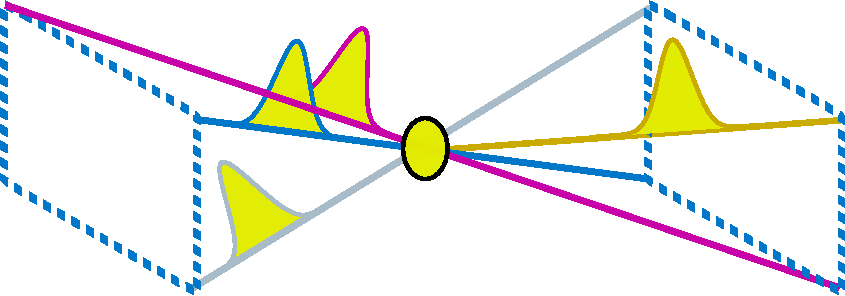
\includegraphics[width=0.8\textwidth]{../figures/FWM_scheme.pdf}
	\caption{Schematic Four-wave mixing setup in a Boxcar geometry. ... \todoimp{Add description. Add S, Add wavevectors, Reduce amplitude of probe pulse.}}
	\label{fig:fwm_box_car_setup}
\end{figure}

\begin{figure}[ht]
	\centering
	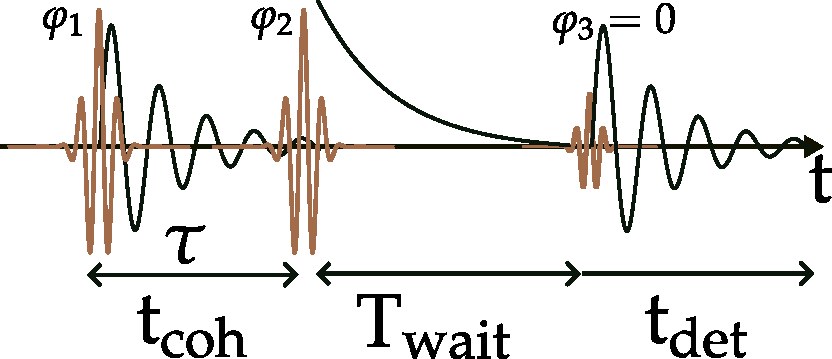
\includegraphics[width=0.8\textwidth]{../figures/FWM_scheme_phase_cycling.pdf}
	\caption{Schematic Four-wave mixing setup. This is the simpler collinear phase-cycling setup, at the cost of requiring multiple measurements with varied pulse phases.
	\todoidea{add ground state at beginning, }}
	\label{fig:fwm_phase_cycling_setup}
\end{figure}

\todoidea{Interaction picture, rotating-wave approximation (introduce but defer justification).}
\todoidea{Also include how to simulate laser pulses:
Gaussian envelope, pulse trains.
1) Time-domain field (carrier × envelope)
$f(t)$ = envelope (e.g. Gaussian $f(t) = \exp\left[-\frac{2\ln 2}{\tau_{\mathrm{FWHM}}^2} t^2\right]$),

$\phi_{\mathrm{CE}}$ = carrier--envelope phase (relevant for few-cycle pulses),

$E_0$ sets peak field (related to pulse energy via the mode area and duration).

Bandwidth for a transform-limited Gaussian:

$\Delta\omega_{\mathrm{FWHM}} \approx \frac{2\ln 2}{\tau_{\mathrm{FWHM}}}$}






\subsection{Heterodyne and Homodyne Detection}
\label{subsec:heterodyne_homodyne}

\noindent There are two main detection schemes used, influencing sensitivity and the information content of the measurements: homodyne and heterodyne detection \cite{abramaviciusetal2009coherentmultidimensionaloptical}.

\noindent In homodyne detection, the intensity of the emitted signal field is measured directly:

\begin{equation}
	S_{\text{HOD}} \propto |E_{\text{S}}|^2 \propto |P^{(3)}|^2
	\label{eq:homodyne}
\end{equation}

\noindent where $E_{\text{S}}$ is the signal electric field and $P^{(3)}$ is the third-order polarization. While experimentally simpler, homodyne detection measures only the signal intensity, losing phase information and it is more susceptible to noise at low signal levels \todoref{find ref}%\cite{abramaviciusetal2009coherentmultidimensionaloptical}.

\noindent Heterodyne detection involves the interference of the signal field with a reference field (local oscillator, LO) of known amplitude and phase:

\begin{equation}
	S_{\text{HET}} \propto |E_{\text{S}} + E_{\text{LO}}|^2 \approx 2\Re{(E_{\text{LO}}^*E_{\text{S}})} + |E_{\text{LO}}|^2 + |E_{\text{S}}|^2
	\label{eq:heterodyne}
\end{equation}

\noindent Since $|E_{\text{LO}}| \gg |E_{\text{S}}|$, the cross-term dominates, and the signal can be extracted by phase-cycling. Heterodyne provides both amplitude and phase information of the signal. The signal scales linearly with the third-order response \todoref{find ref} \todoidea{why is this good?} It also allows for a more direct connection to theoretical models. \todofix{also why?}

\noindent In modern multidimensional spectroscopy, spectral interferometry—a form of heterodyne detection—is widely employed \cite{hybletal1998twodimensionalelectronicspectroscopy}. The signal field and a time-delayed reference pulse are spatially overlapped and spectrally resolved.


\section{Wavevector Phase-Matching Conditions}
\label{sec:phase_matching}

\noindent 
In nonlinear optical processes, multiple light waves interact within a material to generate new frequencies. For these processes to be efficient, the phase relationship between the interacting waves must be maintained throughout the propagation distance. This condition is known as phase-matching.
\noindent 
Like mentioned before, it represents momentum conservation of the incident and outgoing photons. For a general nonlinear process, the wavevector of the generated signal ($\vec{k}_s$) is determined by the vector sum of the input wavevectors:

\begin{equation}
	\vec{k}_s = \pm\vec{k}_1 \pm\vec{k}_2 \pm\vec{k}_3 \pm \ldots
	\label{eq:phase_matching}
\end{equation}

\noindent 
The signs depend on whether the corresponding field acts as a "bra" ($-$) or a "ket" ($+$) in the quantum mechanical description, which corresponds to photon emission or absorption, respectively.

Each laser pulse interacts with the dipole operator $\mu$.
In the rotating-wave approximation (RWA), each field $E_i(t) \propto e^{-i\omega_i t}$ can either:
\todoimp{fact check this:}
Excite the ket side: $\mu_{-} E_i(t) \rightarrow e^{-i\omega_i t} \rightarrow$ forward coherence $e^{-i\omega_{eg} t}$

De-excite the bra side: $\mu_{+} E_i^{*}(t) \rightarrow e^{+i\omega_i t} \rightarrow$ backward (complex-conjugate) coherence $e^{+i\omega_{eg} t}$

That's why the sign in the phase-matching condition ($\pm k_i$) tells you which side of the density matrix the field acted on.

\noindent 
Different combinations of signs correspond to different phase-matching conditions, leading to signals in different spatial directions. These distinct signal directions allow separation of various nonlinear optical processes.


\subsection{Rephasing and nonrephasing Signals}
\label{subsec:rephasing_nonrephasing}

\noindent 
To reduce the number of contributions to the third-order polarization, you can make three vital simplifications: 1.) strict time ordering of the pulses, 2.) the rotating wave approximation (RWA), and 3.) phase-matching \cite{hamm2005principlesnonlinearoptical,  % TODO delete the rest
mukamel1995principlesnonlinearoptical, cho2009twodimensionalopticalspectroscopy, jonas2003twodimensionalfemtosecondspectroscopy}.
For these assumptions, the only surviving terms in the third order polarization are the rephasing and nonrephasing contributions \cite{cho2009twodimensionalopticalspectroscopy, jonas2003twodimensionalfemtosecondspectroscopy}.
\textbf{Rephasing signal} follow the phase-matching condition $\vec{k}_s = -\vec{k}_1 + \vec{k}_2 + \vec{k}_3$. The first interaction creates a coherent superposition between ground and excited states, generated by a complex conjugate interaction of the "bra". The second pulse converts this coherence into a population, and the third pulse generates a new coherence that emits the signal. The phase accumulated due to different frequencies can be reversed during the period between the third interaction and signal emission. This leads to a photon echo effect at $t_{\text{det}} \approx t_{\text{coh}}$ where the dephased components rephase.
This happens for an inhomogeneously broadened ensemble of systems, where different realizations of the system have different transition energies, while the laser pulses drive at constant frequency of $\omega_L$. As a result, some realizations dephase quicker than others. Some realizations should come back in phase around $t_{\text{det}} \approx t_{\text{coh}}$ which is exactly this photon echo.
Contrary to this, \textbf{nonrephasing signal} satisfy $\vec{k}_s = +\vec{k}_1 - \vec{k}_2 + \vec{k}_3$. In this case, the first pulse creates a forward-evolving coherence, and the phase evolution at the third pulse continues in the same direction, and no echo is formed.


\subsection{Phase Cycling in Nonlinear Spectroscopy}
\label{subsec:phase_cycling}

\noindent 
While phase-matching enables the spatial isolation of desired nonlinear Liouville pathways, phase cycling provides an alternative approach by distinguishing signals based on their phases rather than their spatial propagation directions. \todoref{find ref}%\cite{tan2008, yan2009}.
\cite{mukamel1995principlesnonlinearoptical, cho2009twodimensionalopticalspectroscopy, jonas2003twodimensionalfemtosecondspectroscopy, brixneretal2004phasestabilizedtwodimensionalelectronic, greenetal2024vibrationalcoherenceshalfbroadband}.

\noindent 
Here the collinear beam line geometry can be used, simplifying the experimental setup.
This technique is particularly valuable when studying samples without scattering.

\noindent 
And for simulations, as done here, it facilitates the separation of rephasing and nonrephasing signals within the same measurement series.

\noindent 
In phase cycling, multiple measurements are taken with systematically varied phases of the excitation pulses. The desired nonlinear signals can then be extracted through appropriate linear combinations of these measurements. The fundamental principle relies on the fact that different nonlinear pathways respond distinctly to changes in the phases of the input fields.

\noindent 
For a third-order signal generated by three excitation pulses with phases $\phi_1$, $\phi_2$, and $\phi_3$, as seen in Fig. \ref{fig:fwm_phase_cycling_setup}.

\noindent 
By varying the input phases through a complete cycle (in steps of $\pi/2$) and applying discrete Fourier transform to the collected data, specific pathways can be isolated based on their phase dependencies.


\subsection{Phase-Cycling Fourier Selection and Construction of 2D Spectra}
\label{subsec:phase_cycling_fourier_selection}


\noindent 
The nonlinear polarization induced by three incident pulses can be expressed as a Fourier series in the pulse phases $\phi_1, \phi_2, \phi_3$, and individual phase-matched components are isolated via an inverse Fourier transform:

\begin{align}
	P^{(3)}_{n_1,n_2,n_3}(t_{\text{coh}},T,t_{\text{det}}) =
	\frac{1}{(2\pi)^3} \int_{0}^{2\pi}	\int_{0}^{2\pi} \int_{0}^{2\pi}  
	& d\phi_1 d\phi_2 d\phi_3
	e^{-i(n_1\phi_1+n_2\phi_2+n_3\phi_3)} \\
	& P^{(3)}(\phi_1,\phi_2,\phi_3;t_{\text{coh}},T,t_{\text{det}}).
	\label{eq:continuous_phase_cycling}
\end{align}

\noindent 
The physically relevant phase-matching directions correspond to:

\begin{align}
	\vec{k}_{\mathrm{R}}  & = -\vec{k}_1 + \vec{k}_2 + \vec{k}_3,
	                      & (n_1,n_2,n_3)                         & = (-1,+1,+1), \label{eq:rephasing_selection}    \\
	\vec{k}_{\mathrm{NR}} & = +\vec{k}_1 - \vec{k}_2 + \vec{k}_3,
	                      & (n_1,n_2,n_3)                         & = (+1,-1,+1), \label{eq:nonrephasing_selection}
\end{align}

\noindent 
yielding the rephasing (R) and nonrephasing (NR) contributions, respectively.

\noindent 
The (wavevector) phase-matched rephasing signal direction corresponds to selecting the Fourier index triple $(n_1,n_2,n_3)=(-1,+1,+1)$, while the nonrephasing direction corresponds to $(+1,-1,+1)$ \cite{mukamel1995principlesnonlinearoptical, cho2009twodimensionalopticalspectroscopy, greenetal2024vibrationalcoherenceshalfbroadband}.

\noindent 
The emitted field in a given phase-matching direction is proportional to the corresponding polarization:

\begin{equation}
	E_{k_s}(t_{\text{coh}},T,t_{\text{det}}) \propto i P_{\vec{k}_S}(t_{\text{coh}},T,t_{\text{det}}).
	\label{eq:field_polarization_relation}
\end{equation}


\paragraph{Time--Frequency Transforms.}

\noindent 
After phase selection, the third order complex time-domain field $E_{k_S}(t_{\text{coh}}, T, t_{\text{det}})$ is Fourier transformed over the detection time $t_{\text{det}}$ and the coherence time $t_{\text{coh}}$ to construct the two-dimensional spectra (cf. Eq.~\eqref{eq:2des_signal}):

\begin{align}
	S_{R}(\omega_{\text{coh}}, T, \omega_{\text{det}})
	 & =
	\int dt_{\text{coh}} \int dt_{\text{det}} \;
	e^{+ i \omega_{\text{coh}} t_{\text{coh}}} e^{- i \omega_{\text{det}} t_{\text{det}}}
	E_{R}(t_{\text{coh}}, T, t_{\text{det}}),
	\label{eq:rephasing_transform} \\
	S_{NR}(\omega_{\text{coh}}, T, \omega_{\text{det}})
	 & =
	\int dt_{\text{coh}} \int dt_{\text{det}} \;
	e^{- i \omega_{\text{coh}} t_{\text{coh}}} e^{- i \omega_{\text{det}} t_{\text{det}}}
	E_{NR}(t_{\text{coh}}, T, t_{\text{det}}),
	\label{eq:nonrephasing_transform}
\end{align}

\noindent 
where $E(t_{\text{coh}}, T, t_{\text{det}})$ is the time-domain electrical signal field.

\noindent 
The opposite sign in the $t_{\text{coh}}$-exponent implements the standard convention distinguishing rephasing (photon-echo) and nonrephasing contributions \cite{cho2009twodimensionalopticalspectroscopy, greenetal2024vibrationalcoherenceshalfbroadband}. In discrete numerical implementations, Eqs.~\eqref{eq:rephasing_transform}--\eqref{eq:nonrephasing_transform} are approximated by (shifted) fast Fourier transforms \cite{cho2009twodimensionalopticalspectroscopy, greenetal2024vibrationalcoherenceshalfbroadband}.

\paragraph{Global Phase and Absorptive Combination.}

\noindent 
The experimentally measured (or simulated) complex spectra $S_{R}$ and $S_{NR}$ can be combined to  construct the purely absorptive 2D spectrum \cite{mukamel1995principlesnonlinearoptical, jonas2003twodimensionalfemtosecondspectroscopy, greenetal2024vibrationalcoherenceshalfbroadband}
\begin{equation}
	S_{\text{abs}}(\omega_{\text{coh}}, T, \omega_{\text{det}})
	=
	\Re \left\{
	S_{R}(\omega_{\text{coh}}, T, \omega_{\text{det}}) + S_{NR}(\omega_{\text{coh}}, T, \omega_{\text{det}})
	\right\}.
	\label{eq:absorptive_spectrum}
\end{equation}

\noindent 
The absorptive spectra is free from broadening refractive contributions \cite{fullerogilvie2015experimentalimplementationstwodimensional}.



%----------------------------------------------------------------------------------------
%	SECTION 4: PHOTON ECHO SPECTROSCOPY
%----------------------------------------------------------------------------------------
\section{Photon Echo Spectroscopy}
\label{sec:photon_echo}
\noindent 
The echo intensity as a function of the delay time $t_{\text{coh}}$ reveals information about the dephasing processes in the system.

\noindent 
It is important to emphasize that static inhomogeneity is crucial for the appearance of the photon echo signal. This inhomogeneity arises from variations in the local environment of individual quantum systems within the ensemble, leading to a distribution of transition frequencies. In this thesis, in the numerical simulations, static inhomogeneity is taken into account by averaging the results over an ensemble of different realizations of the Hamiltonian \cite{cho2009twodimensionalopticalspectroscopy, mukamel1995principlesnonlinearoptical}. Without this inhomogeneous distribution, all systems would evolve identically, and the characteristic echo phenomenon would not occur.

\noindent 
By scanning the waiting time $T$, this technique allows measurement of population dynamics and spectral diffusion processes.

\subsection{Two-Dimensional Electronic Spectroscopy}
\label{subsec:2d_spectroscopy}

\noindent 
It correlates excitation and detection frequencies, revealing couplings between different transitions and energy transfer pathways.

\noindent 
Recall that a complete 2D spectrum is built from repeated three-pulse sequences while the coherence time $t_{\text{coh}}$ is scanned. The rephasing photon-echo signal arises after a finite rephasing time $t$ for sequences in which pulse 1 precedes pulse 2 ($t_{\text{coh}}>0$) and is recorded in the phase-matched direction $-\vec{k}_1 + \vec{k}_2 + \vec{k}_3$. As discussed in Subsec.~\ref{subsec:rephasing_nonrephasing}, the ground–excited coherences during $t_{\text{coh}}$ and $t$ accumulate opposite phases in the rephasing branch. When the ordering of pulses 1 and 2 is reversed ($t_{\text{coh}}<0$), these phase factors add rather than cancel, yielding a nonrephasing free-induction–decay signal that emerges immediately following pulse 3; this contribution provides information complementary to the rephasing branch \cite{ginsbergetal2009twodimensionalelectronicspectroscopy}.

\noindent The resulting 2D spectrum contains peaks along the diagonal ($\omega_{\text{coh}} = \omega_{\text{det}}$) corresponding to the linear absorption spectrum, while off-diagonal peaks reveal couplings and energy transfer between different states. The evolution of the 2D spectra with waiting time $T$ provides detailed information about energy transfer kinetics, spectral diffusion, and quantum coherence effects.

\subsection{Applications of Photon Echo Spectroscopy}
\label{subsec:echo_applications}

\noindent Photon echo techniques have been applied to a wide range of problems across chemistry, biology, and materials science:

\textbf{Exciton dynamics} in photosynthetic complexes, revealing quantum coherent energy transfer pathways \todoref{find ref}%\cite{engel2007, schlau-cohen2011}
\textbf{Vibrational dynamics} in proteins and liquids, elucidating structural fluctuations and hydrogen-bonding networks \cite{hammzanni2011conceptsmethods2d}
\textbf{Charge transfer processes} in organic photovoltaics and light-harvesting systems
\textbf{Coupling mechanisms} between electronic and vibrational degrees of freedom \cite{khaliletal2004vibrationalcoherencetransfer}



%----------------------------------------------------------------------------------------
\todoidea{

2. Regroup / Change Order
3. Improvements
To make the chapter a stronger foundation, enhance clarity, relevance, and connections to your thesis. Focus on electronic spectroscopy, open quantum systems (e.g., dephasing, dissipation), and biological contexts (e.g., microtubules as complex open systems). Add transitions between sections for better flow.

Add Thesis-Specific Emphasis: Throughout, weave in connections to open quantum systems (e.g., in "Energy Dissipation," link to Lindblad operators or bath interactions). In "Two-Dimensional Electronic Spectroscopy," explicitly state how 2DES reveals couplings and dynamics in systems like microtubules. Add a forward-looking paragraph in the intro/outro noting how this chapter sets up your modeling work.

Improve Mathematical Rigor and Clarity: Equations are good, but add brief explanations of their relevance (e.g., after Eq. 2.1, note how it applies to electronic transitions). For complex sections like phase cycling, use more figures or diagrams (you already have a TODO for one). Ensure notation consistency (e.g., use $\omega$ for angular frequency uniformly).

Enhance Biological Relevance: In "Applications," expand on exciton dynamics in photosynthetic systems as analogs to microtubule coherence. Add a subsection or paragraph on "Towards Biological Systems" at the end, discussing how 2DES can probe quantum effects in cytoskeletal structures.

Strengthen References and Citations: You have many TODOs for refs—prioritize adding them, especially for 2DES and open systems (e.g., cite Mukamel for nonlinear optics, and papers on biological 2DES). Ensure citations align with your thesis's scope.

Improve Flow and Language: Add transitional sentences (e.g., "Building on these fundamentals, we now explore nonlinear optics..."). Use active voice and concise language. Fix minor issues like inconsistent capitalization (e.g., "Rephasing" vs. "rephasing").

Add Figures and Examples: You have a TODO for a figure in phase cycling—add it. Include simple examples (e.g., a toy model of electronic transitions in a two-level system) to illustrate points.

Overall Cohesion: End with a strong conclusion summarizing how these principles underpin your thesis's modeling of microtubules. This reinforces the chapter as a foundation.}
%% !TEX root = ../main.tex
\chapter{Model Systems}

\label{chapter_model_systems}

Having developed the two-dimensional spectroscopic formalism and open-system dynamics earlier, we now transition to applying the photon-echo spectroscopy workflow to concrete models. We start from minimal reference systems (a single qubit and a four-level system formed by two coupled qubits) and then generalize to $N$ qubits arranged on a cylindrical geometry, mirroring the architectural motifs of microtubules where each site represents a bonding location in the molecular scaffold \cite{kalraetal2023electronicenergymigration}. Throughout, we connect to standard third-order spectroscopy concepts \cite{mukamel1995principlesnonlinearoptical,jonas2003twodimensionalfemtosecondspectroscopy,cho2009twodimensionalopticalspectroscopy} and use the master-equation tools introduced previously (see Chapter~\ref{chapter_open_quantum_systems}; cf. \cite{breuerpetruccione2009theoryopenquantum,redfield1965theoryrelaxationprocesses}).

%-------------------------------------------------------------------------------
%	SECTION 1: REFERENCE MODELS
%-------------------------------------------------------------------------------

\section{Reference Models}

\subsection{Qubit Model}
Single two-level systems (spin–boson model) are the canonical testbed in open-quantum-system theory; their weak-coupling dynamics under Redfield and Lindblad-type generators are well characterized \cite{redfield1965theoryrelaxationprocesses,breuerpetruccione2009theoryopenquantum,manzano2020shortintroductionlindblad,campaiolietal2024quantummasterequations}, with standard choices of bath spectral densities (e.g., Ohmic or Drude–Lorentz) \cite{ritscheleisfeld2014analyticrepresentationsbath}. As a representative study, polarization-resolved dephasing and relaxation of a qubit coupled to a bosonic bath has been analyzed within Redfield theory in \cite{palmnalbach2019dephasingrelaxationalpolarized}, providing a useful baseline against which to benchmark our spectroscopy workflow.

The qubit system Hamiltonian is given by $H_{\mathrm{S}} = \frac{\omega}{2} \sigma_z$, or equivalently
\begin{align}
	H_{\mathrm{S}} & = \omega \ket{e}\bra{e} ,
	\label{eq:qubit_system}
\end{align}
where $\omega$ is the qubit transition frequency, $\sigma_z$ is the Pauli operator in z direction.
The environment is characterized by a spectral density $J(\omega)$ (cf. \cite{breuerpetruccione2009theoryopenquantum,ritscheleisfeld2014analyticrepresentationsbath}). In the photon-echo context, the system-field interaction in the dipole approximation enters the third-order response, while the reduced dynamics may be propagated with the Redfield or Lindblad-type generators derived in Chapter~\ref{chapter_open_quantum_systems} (see also \cite{campaiolietal2024quantummasterequations,manzano2020shortintroductionlindblad}).

For spectroscopy, we assume a system dipole operator $\hat{\mu}_{\mathrm{S}} = \mu\,\sigma_x$ (oriented relative to the laboratory frame by the polarization geometry), and compute the rephasing and nonrephasing third-order signals using the response-function formalism \cite{mukamel1995principlesnonlinearoptical,jonas2003twodimensionalfemtosecondspectroscopy}.

\todoidea{explain that this simplest two level system only offers limited insights, but is a good test case for the workflow. This is due to the lack of multiple states and pathways, which are essential for capturing the rich dynamics and interactions detectable with 2D spectroscopy.}

\todoidea{move this to the model chapter}
\subsection{Four-Level System Model for Third-Order Spectroscopy}
\label{subsec:four_level_model}

\noindent While two-level systems suffice for linear spectroscopy and basic nonlinear responses, additional states must be included to account for processes such as excited-state absorption. A commonly used minimal pedagogical model is a four-level system (ground, two single-excited, and one double-excited state), which allows all major third-order Liouville pathways to be represented\cite{cho2009twodimensionalopticalspectroscopy, abramaviciusetal2009coherentmultidimensionaloptical}.

\noindent In a four-level system, the energy states include:

\begin{itemize}
	\item $|g\rangle$: Ground state
	\item $|e_1\rangle$ and $|e_2\rangle$: First excited states (single excitons)
	\item $|f\rangle$: Doubly excited state (two excitons)
\end{itemize}

\noindent This configuration allows modeling of all possible Liouville pathways that contribute to the third-order response function \cite{mukamel1995principlesnonlinearoptical}. The inclusion of multiple excited states and a doubly excited state is essential for describing phenomena such as ground-state bleaching, stimulated emission, and excited-state absorption—the three primary components of signals observed in techniques like transient absorption and 2D electronic spectroscopy.

\noindent The third-order polarization $P^{(3)}$ in such a system can be expressed as a sum of different pathways:

\begin{equation}
	P^{(3)} = P^{(3)}_{GSB} + P^{(3)}_{SE} + P^{(3)}_{ESA} + \ldots
	\label{eq:third_order_contributions}
\end{equation}

\noindent where GSB, SE, and ESA represent ground-state bleaching, stimulated emission, and excited-state absorption, respectively. The line-broadening function formalism within this four-level model enables detailed analysis of spectral lineshapes and system-bath interactions \cite{cho2009twodimensionalopticalspectroscopy, abramaviciusetal2009coherentmultidimensionaloptical}.

\noindent While two-level systems are pedagogically valuable and simplify certain calculations, the four-level model captures the richness of nonlinear spectroscopic signals and serves as the foundation for interpreting complex experiments such as multidimensional spectroscopy.


\subsection{4-Level System (Two Qubits)}

Extending one qubit to two coupled qubits, we obtain a four-level manifold spanned by $\{\ket{gg},\ket{ge},\ket{eg},\ket{ee}\}$. A convenient system Hamiltonian is
\begin{equation}
	H_{\mathrm{S}}^{\,(2)} = \sum_{i=1}^{2} \frac{\omega_i}{2}\, \sigma_z^{(i)}
	\,+ J\,\bigl( \sigma_{+}^{(1)}\sigma_{-}^{(2)} + \sigma_{-}^{(1)}\sigma_{+}^{(2)} \bigr),
	\label{eq:two_qubit_system}
\end{equation}
with coherent exchange coupling $J$. For open dynamics we consider independent local baths,
\begin{equation}
	H_{\mathrm{B}}^{\,(2)} = \sum_{i=1}^{2} \sum_{k} \omega_{k,i}\, a_{k,i}^{\dagger} a_{k,i},
	\quad
	H_{\mathrm{SB}}^{\,(2)} = \sum_{i=1}^{2} \sum_{k} g_{k,i}\,\bigl( \sigma_{+}^{(i)} a_{k,i} + \sigma_{-}^{(i)} a_{k,i}^{\dagger} \bigr),
	\label{eq:two_qubit_bath}
\end{equation}
though correlated baths can be accommodated as discussed in Chapter~\ref{chapter_open_quantum_systems}. This minimal dimer already exhibits cross-peaks and coherence transfer in photon-echo spectra \cite{pisliakovetal2006twodimensionalopticalthreepulse}, making it a natural benchmark for the workflow.

%-------------------------------------------------------------------------------
%	SECTION 2: N QUBITS ON CYLINDRICAL GEOMETRY
%-------------------------------------------------------------------------------

\section{Generalization to \texorpdfstring{$N$}{N} Qubits on Cylindrical Geometry}

Motivated by the protofilament arrangement in microtubules, we place $N$ qubits on a discretized cylindrical surface. The interaction energy of two such sites is given by isotropic dipole couplings of the form \cite{griffiths2013introductionelectrodynamics}
\begin{equation}
	J_{ij} \propto \frac{1}{ \lVert \vec{r}_{ij} \rVert^{3} }
	\left[
		\vec{\mu}_i \cdot \vec{\mu}_j - 3\,(\vec{\mu}_i \cdot \hat{\vec{r}}_{ij})(\vec{\mu}_j \cdot \hat{\vec{r}}_{ij})
		\right],
	\label{eq:dipole_dipole}
\end{equation}
where $\vec{\mu}_i$ are transition dipoles and $\vec{r}_{ij}$ the displacement between sites $i$ and $j$ (cf. \cite{lehmberg1970radiationatomsystem,masters2014pathsforstersresonance}).

Let $N_{\theta}$ be the number of sites per ring and $N_{z}$ the number of rings (so $N = N_{\theta} N_{z}$). We index sites by $(m,n)$ with $m\in\{0,\dots,N_{\theta}-1\}$ (azimuthal) and $n\in\{0,\dots,N_{z}-1\}$ (axial). The system Hamiltonian reads
\begin{align}
	H_{\mathrm{S}}^{\,(N)} = & \sum_{n=1}^{N} \omega_{n} \ket{n}\bra{n} + \sum_{m<n}^{N} J_{mn} \bigl( \sigma_{+}^{(m)} \sigma_{-}^{(n)} + \mathrm{h.c.} \bigr) \\
	                         & + \sum_{m<n}^{N} (\omega_{m} + \omega_{n}) \ket{m, n}\bra{m, n}
	+ \sum_{m n l}^{N} \bigl[ \bigl( J_{ml} \ket{ln}\bra{mn}
		+ J_{nl} \ket{lm}\bra{mn} \bigr) + \mathrm{h.c.} \bigr]
	\label{eq:Nqubit_hamiltonian}
\end{align}
implementing periodic boundary conditions in the azimuthal direction.

The bath part may be modeled as independent local environments,
\begin{equation}
	H_{\mathrm{B}}^{\,(N)} = \sum_{m,n} \sum_{k} \omega_{k,(m,n)} a_{k,(m,n)}^{\dagger} a_{k,(m,n)},
	\quad
	H_{\mathrm{SB}}^{\,(N)} = \sum_{m,n} \sum_{k} g_{k,(m,n)}\,\bigl( \sigma_{+}^{(m,n)} a_{k,(m,n)} + \mathrm{h.c.} \bigr),
	\label{eq:Nqubit_bath}
\end{equation}
with spectral densities chosen to reflect protein or solvent environments \cite{rodenetal2012accountingintramolecularvibrational,ritscheleisfeld2014analyticrepresentationsbath}.

This geometry captures collective transport pathways and their photon-echo signatures, offering a route to connect microscopic couplings to observed energy migration along microtubules \cite{kalraetal2023electronicenergymigration}. It also allows us to compare rephasing/nonrephasing features and waiting-time dynamics against the reference dimer, thereby isolating geometric versus environmental contributions \cite{mukamel1995principlesnonlinearoptical,segarra-martietal2018accuratesimulationtwodimensional}.
%\include{chapters/todo_example}

\iffalse
	# comment out everything below this line
\fi
%-------------------------------------------------------------------------------
%	APPENDICES
%-------------------------------------------------------------------------------

\appendix

%\include{appendices/_template_appendix} % corrected appendix path

%-------------------------------------------------------------------------------
%	BIBLIOGRAPHY
%-------------------------------------------------------------------------------

\printbibliography

\end{document}
% IDEA ABOUT HOW TO STRUCTURE THE THESIS
%https://chatgpt.com/share/686e2740-d700-8009-8b73-fc47a1730560